\section{Data visualization and exploration}
\setcounter{figure}{0}

\subsection{Data extraction}

Generally, we have a bunch of different data sources, with a multitude of different standards, features, and also information that can be extracted. The general problem is depicted in \ref{fig:2_data_extraction}.

\begin{figure}[H]
  \centering
  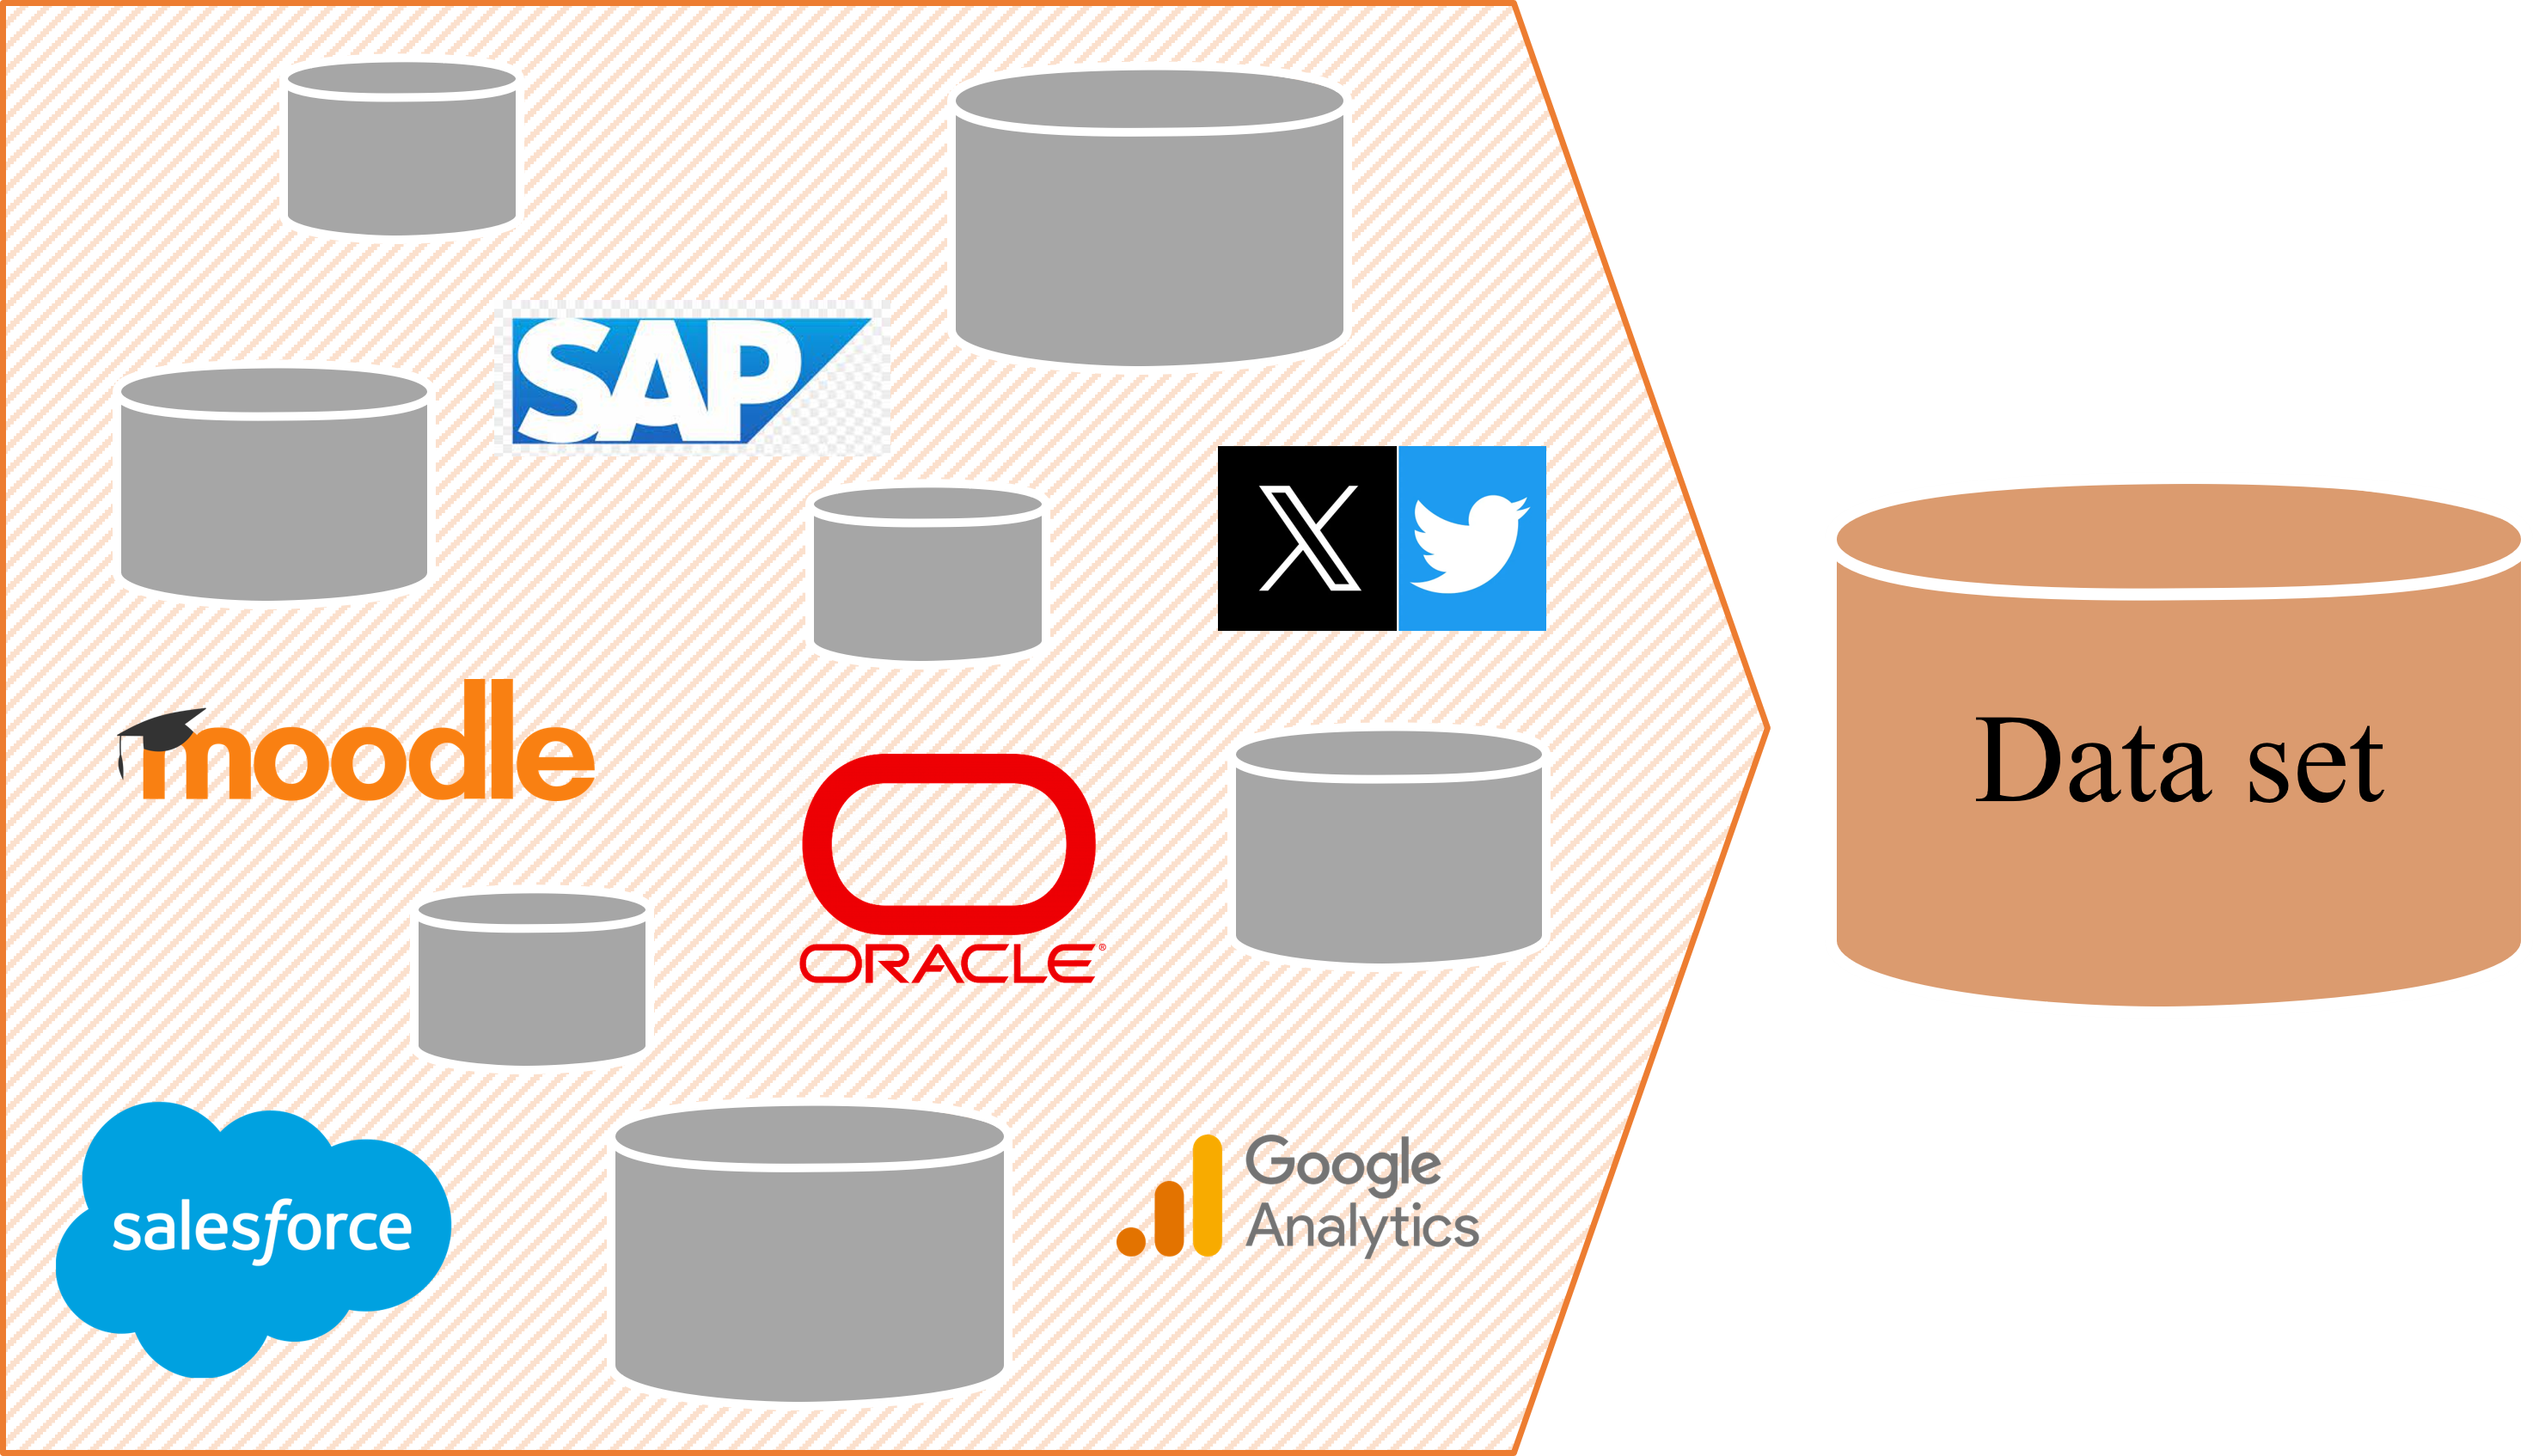
\includegraphics[width=0.4\textwidth]{assets/visualization_and_extraction/data_extraction.png}
  \caption{Data extraction from different sources}
  \label{fig:2_data_extraction}
\end{figure}

The different datatypes were already analyzed in the previous chapter, but still \ref{fig:2_data_types} shows a quick recap. Important to mention, that any unstructured data is considered a bit stream.

\begin{figure}[H]
  \centering
  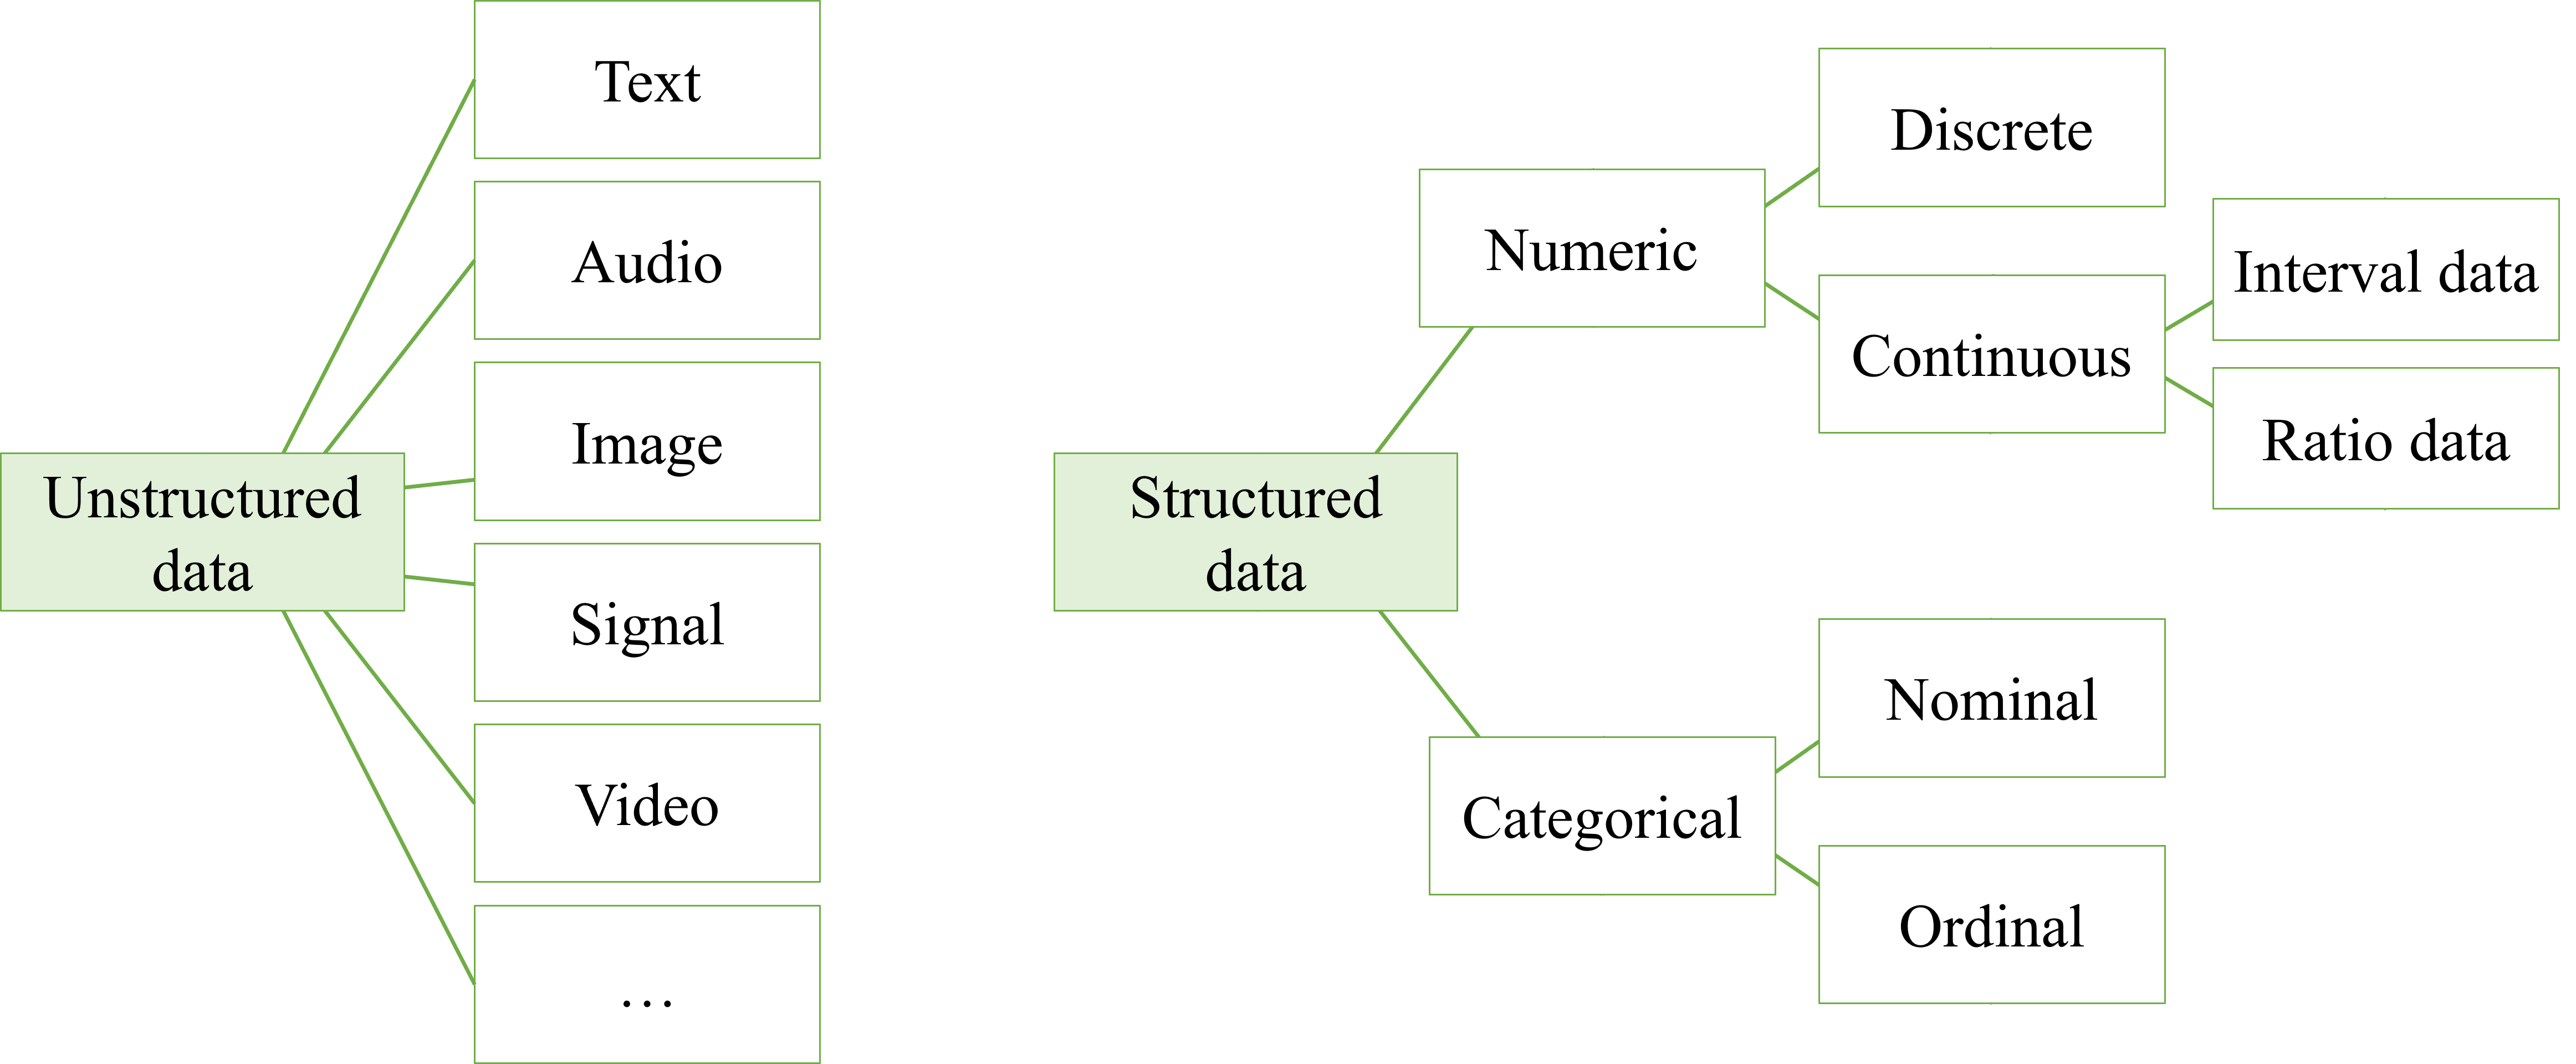
\includegraphics[width=0.7\textwidth]{assets/visualization_and_extraction/data_types.png}
  \caption{Recap: overview types of data}
  \label{fig:2_data_types}
\end{figure}

Important when wanting to obtain any object is of course the feature extraction. The data described by features are usually captured in a tabular form, with rows as the instances and columns as the features. There exist some special features:
\begin{itemize}
  \item \textbf{Time} usually always plays a role in data observation, which is why it is usually one of the recorded features.
  \item Then there are also the \textbf{target features}, in contrast to the descriptive features. The concept was introduced in the last section as part of supervised learning.
\end{itemize}


\subsection*{Importance of visualization}
We now looked at how we can represent our data in a very machine-friendly represented way. The following subsection shows, why visualization of data has any importance, even though tabular data already captures the features nicely.

It is important as a human to explore your data before applying mathematical operations to see, which techniques make sense to apply to the provided data. As an extreme example, we will take a look at \textbf{Anscombe's quartet} created by Francis Anscombe in 1973. 
\begin{itemize}
  \item You can see the raw data of all four datasets in the table in \ref{fig:2_anscombes_quartet}. Since the format isn't human-friendly to read, you might not see any significant differences in the data.
  \item Now consider applying the evaluation depicted below the data table. As you can see: all of the properties that are evaluated are exactly the same for all datasets.
  \item BUT, if you visualize the datasets, e.g. as simple scatter plots, you see, how drastically they vary. These show the importance of first exploring your data, to then have a better evaluation foundation for the applied techniques.
\end{itemize} 

\begin{figure}[H]
  \centering
  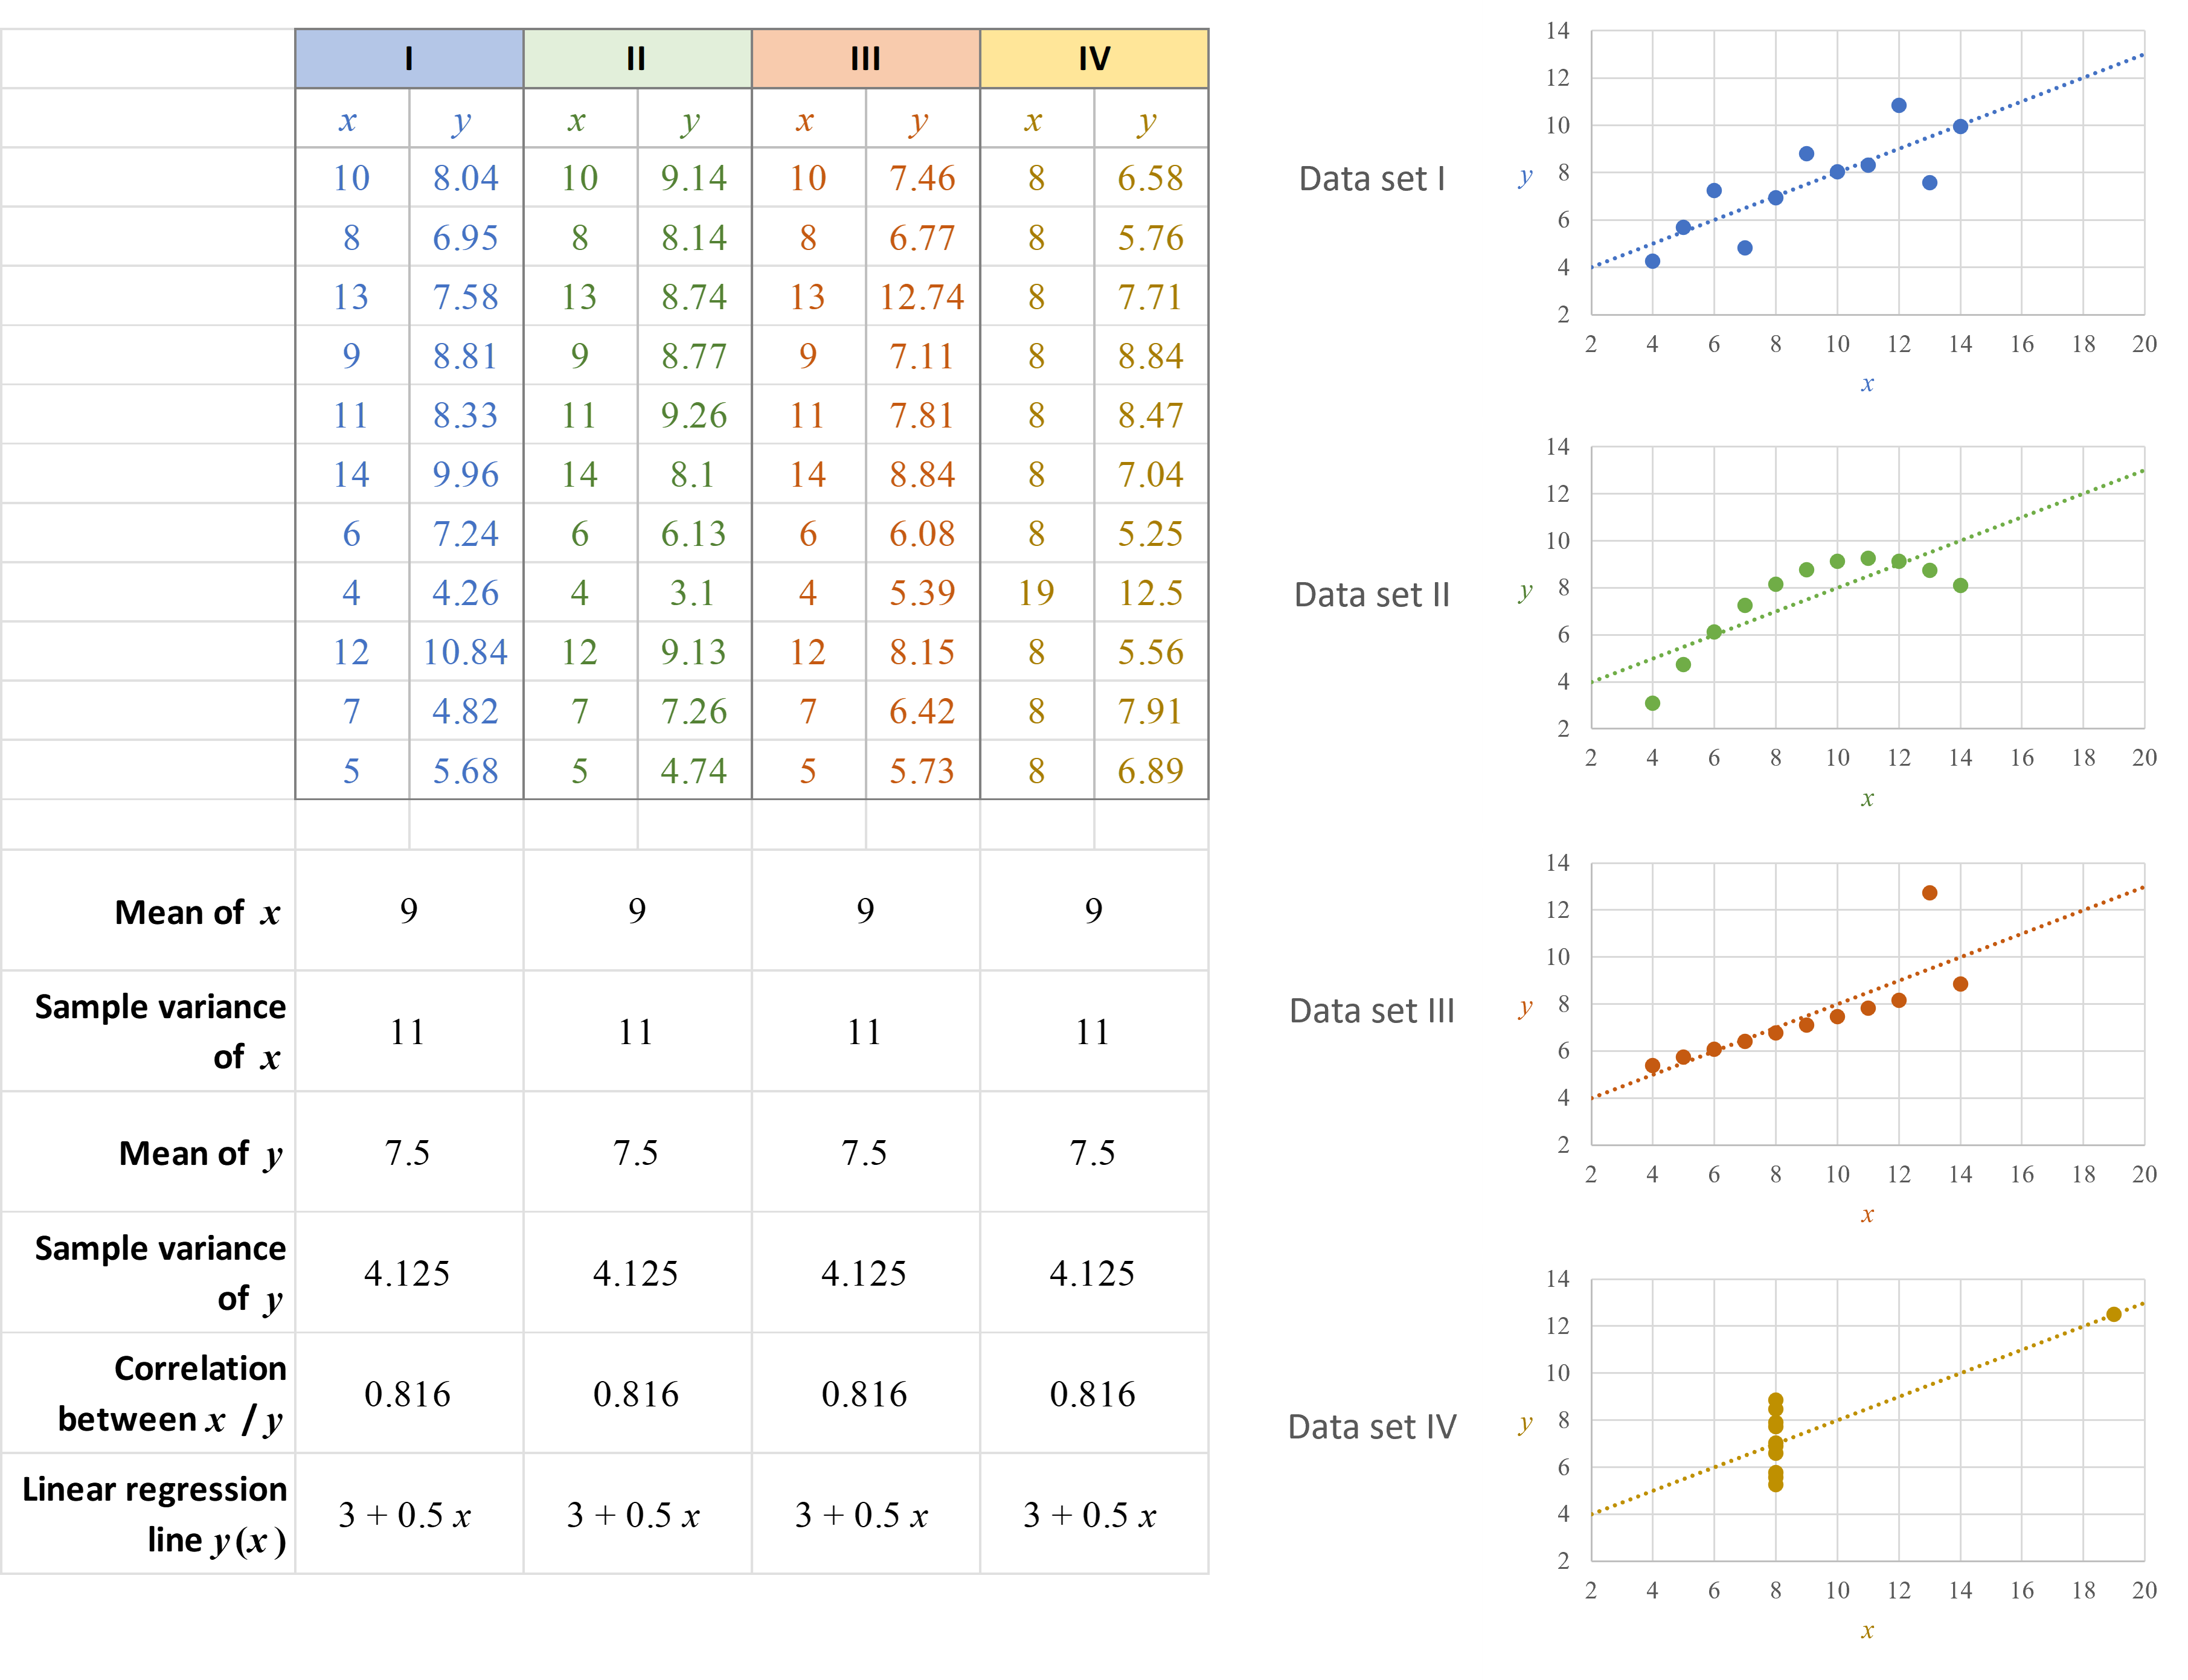
\includegraphics[width=\textwidth]{assets/visualization_and_extraction/anscombes_quartet.png}
  \caption{Anscombes quartet}
  \label{fig:2_anscombes_quartet}
\end{figure}

The next example highlighting the importance of visualization and especially of a fitting and well-thought-out visualization is the diagram as shown in \ref{fig:2_napoleon}. The chart shows the following aspects, which are quite a lot, while still keeping a good overview:
\begin{itemize}
  \item The number of men in Napoleon's 1812 Russian campaign army,
  \item Their movements (direction),
  \item The temperature encountered on the return path,
  \item All given a specific geographic point.
\end{itemize}

\begin{figure}[H]
  \centering
  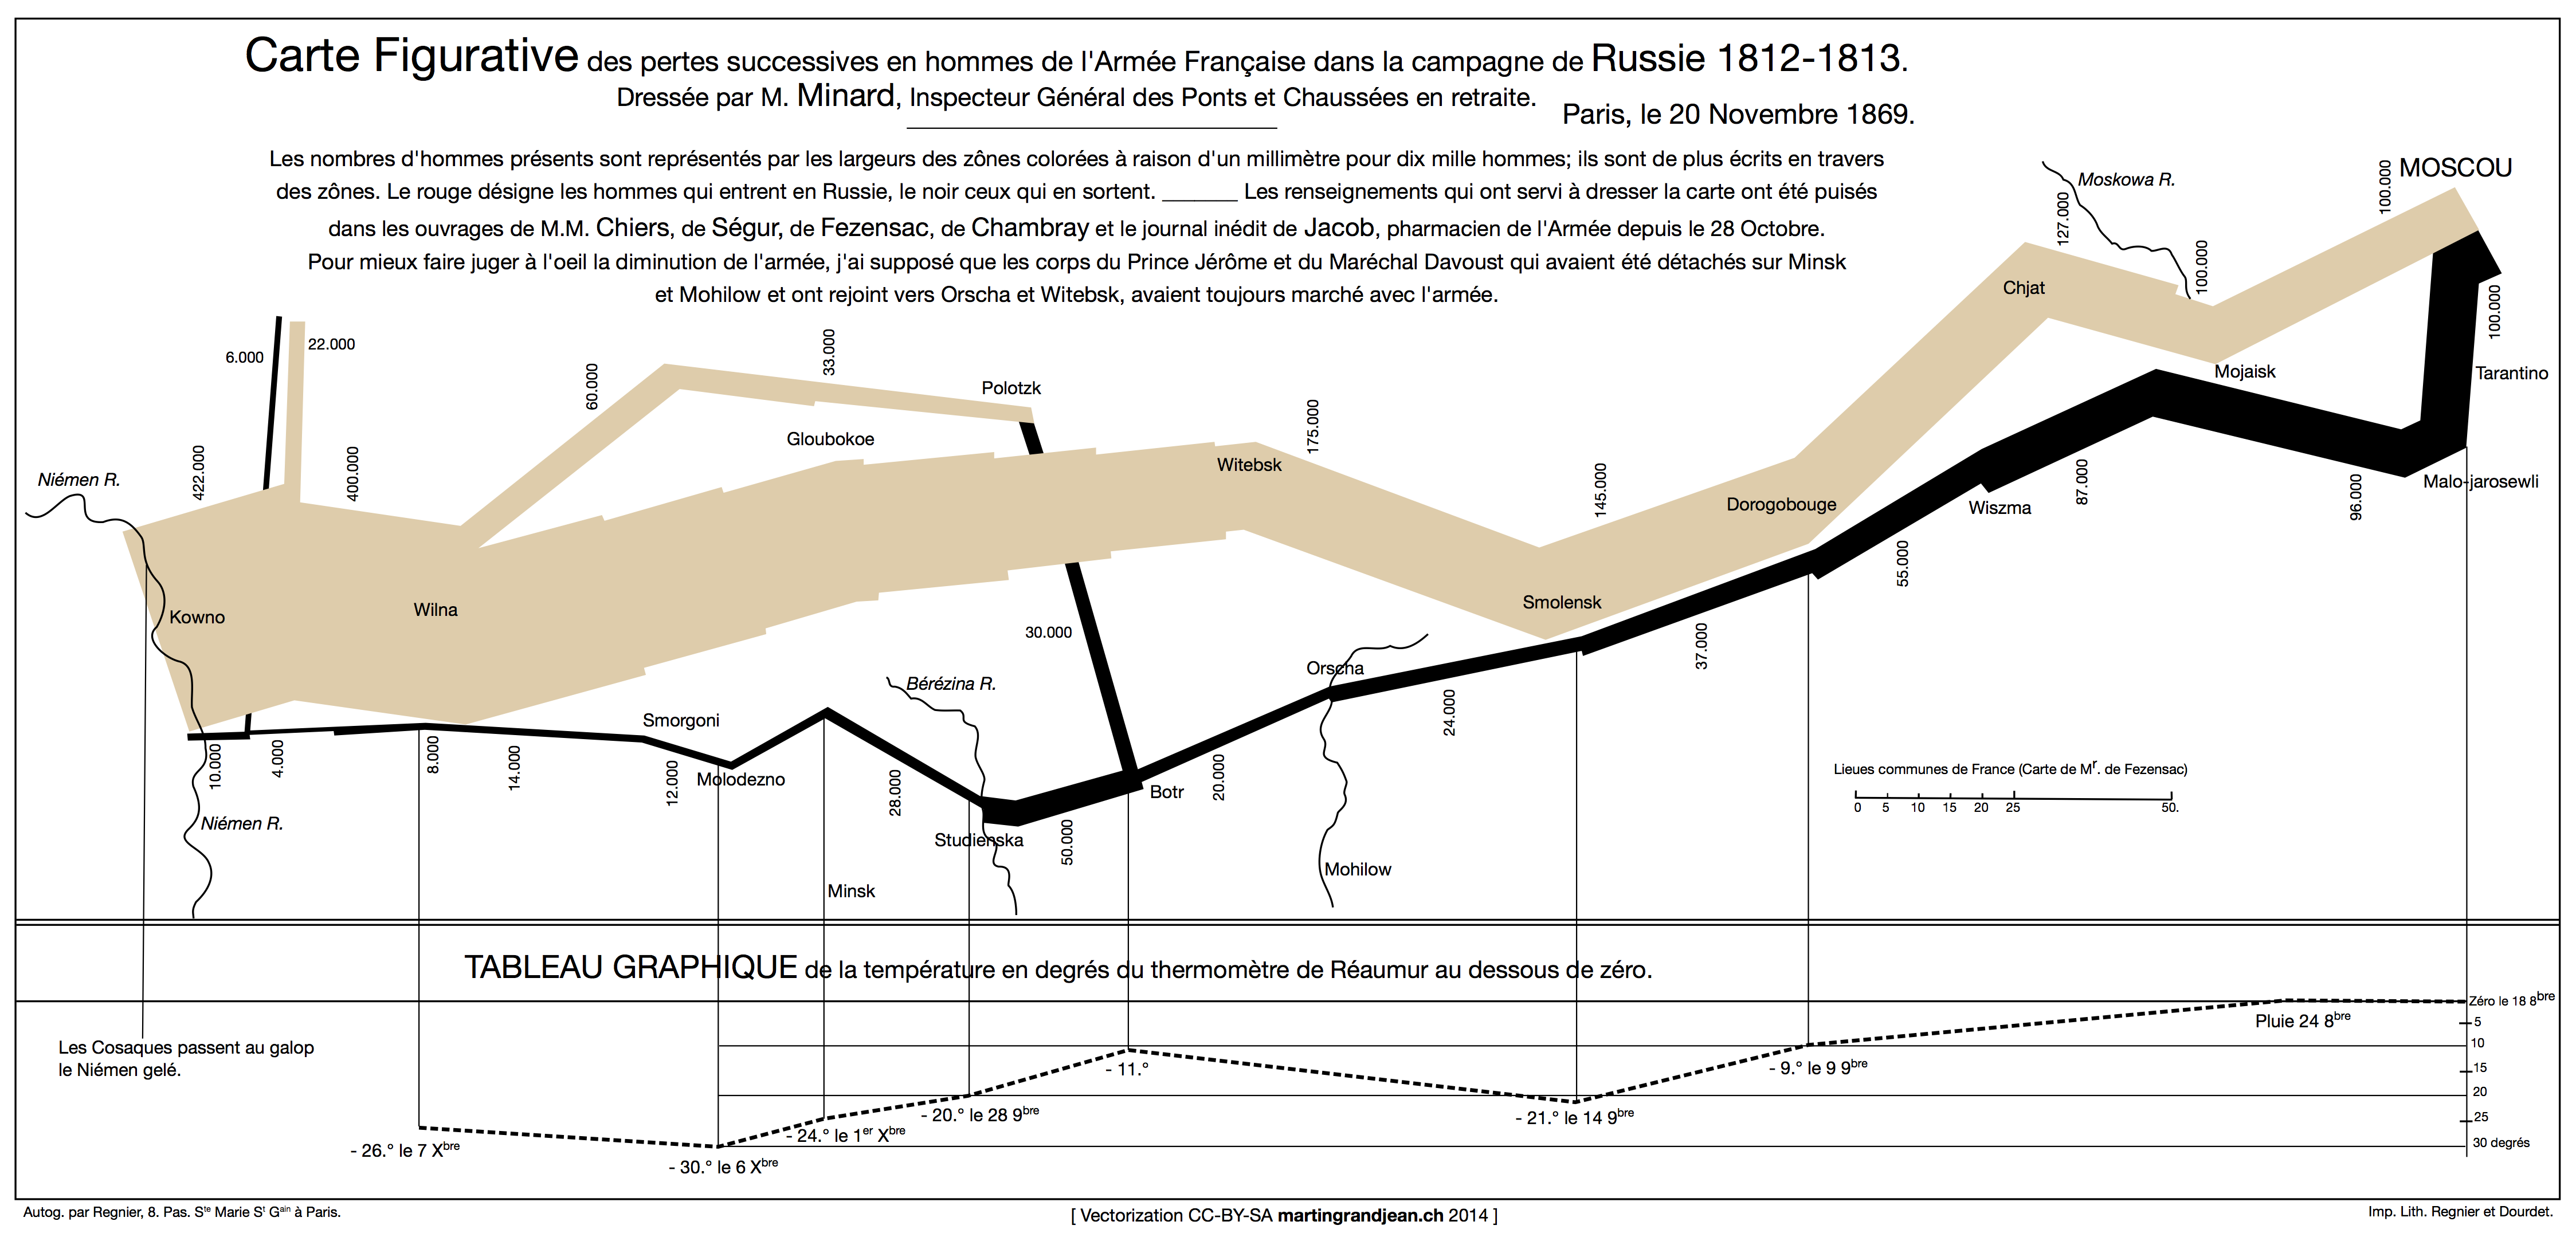
\includegraphics[width=\textwidth]{assets/visualization_and_extraction/napolean.png}
  \caption{Multi-feature visualization (Napoleon's army)}
  \label{fig:2_napoleon}
\end{figure}

As a final example: when we have given different event data, it often helps to plot this in some way as can be seen in \ref{fig:2_event_data}. With the visualization, some sort of trend, similarities, certain batching areas, etc. can be directly seen.

\begin{figure}[H]
  \centering
  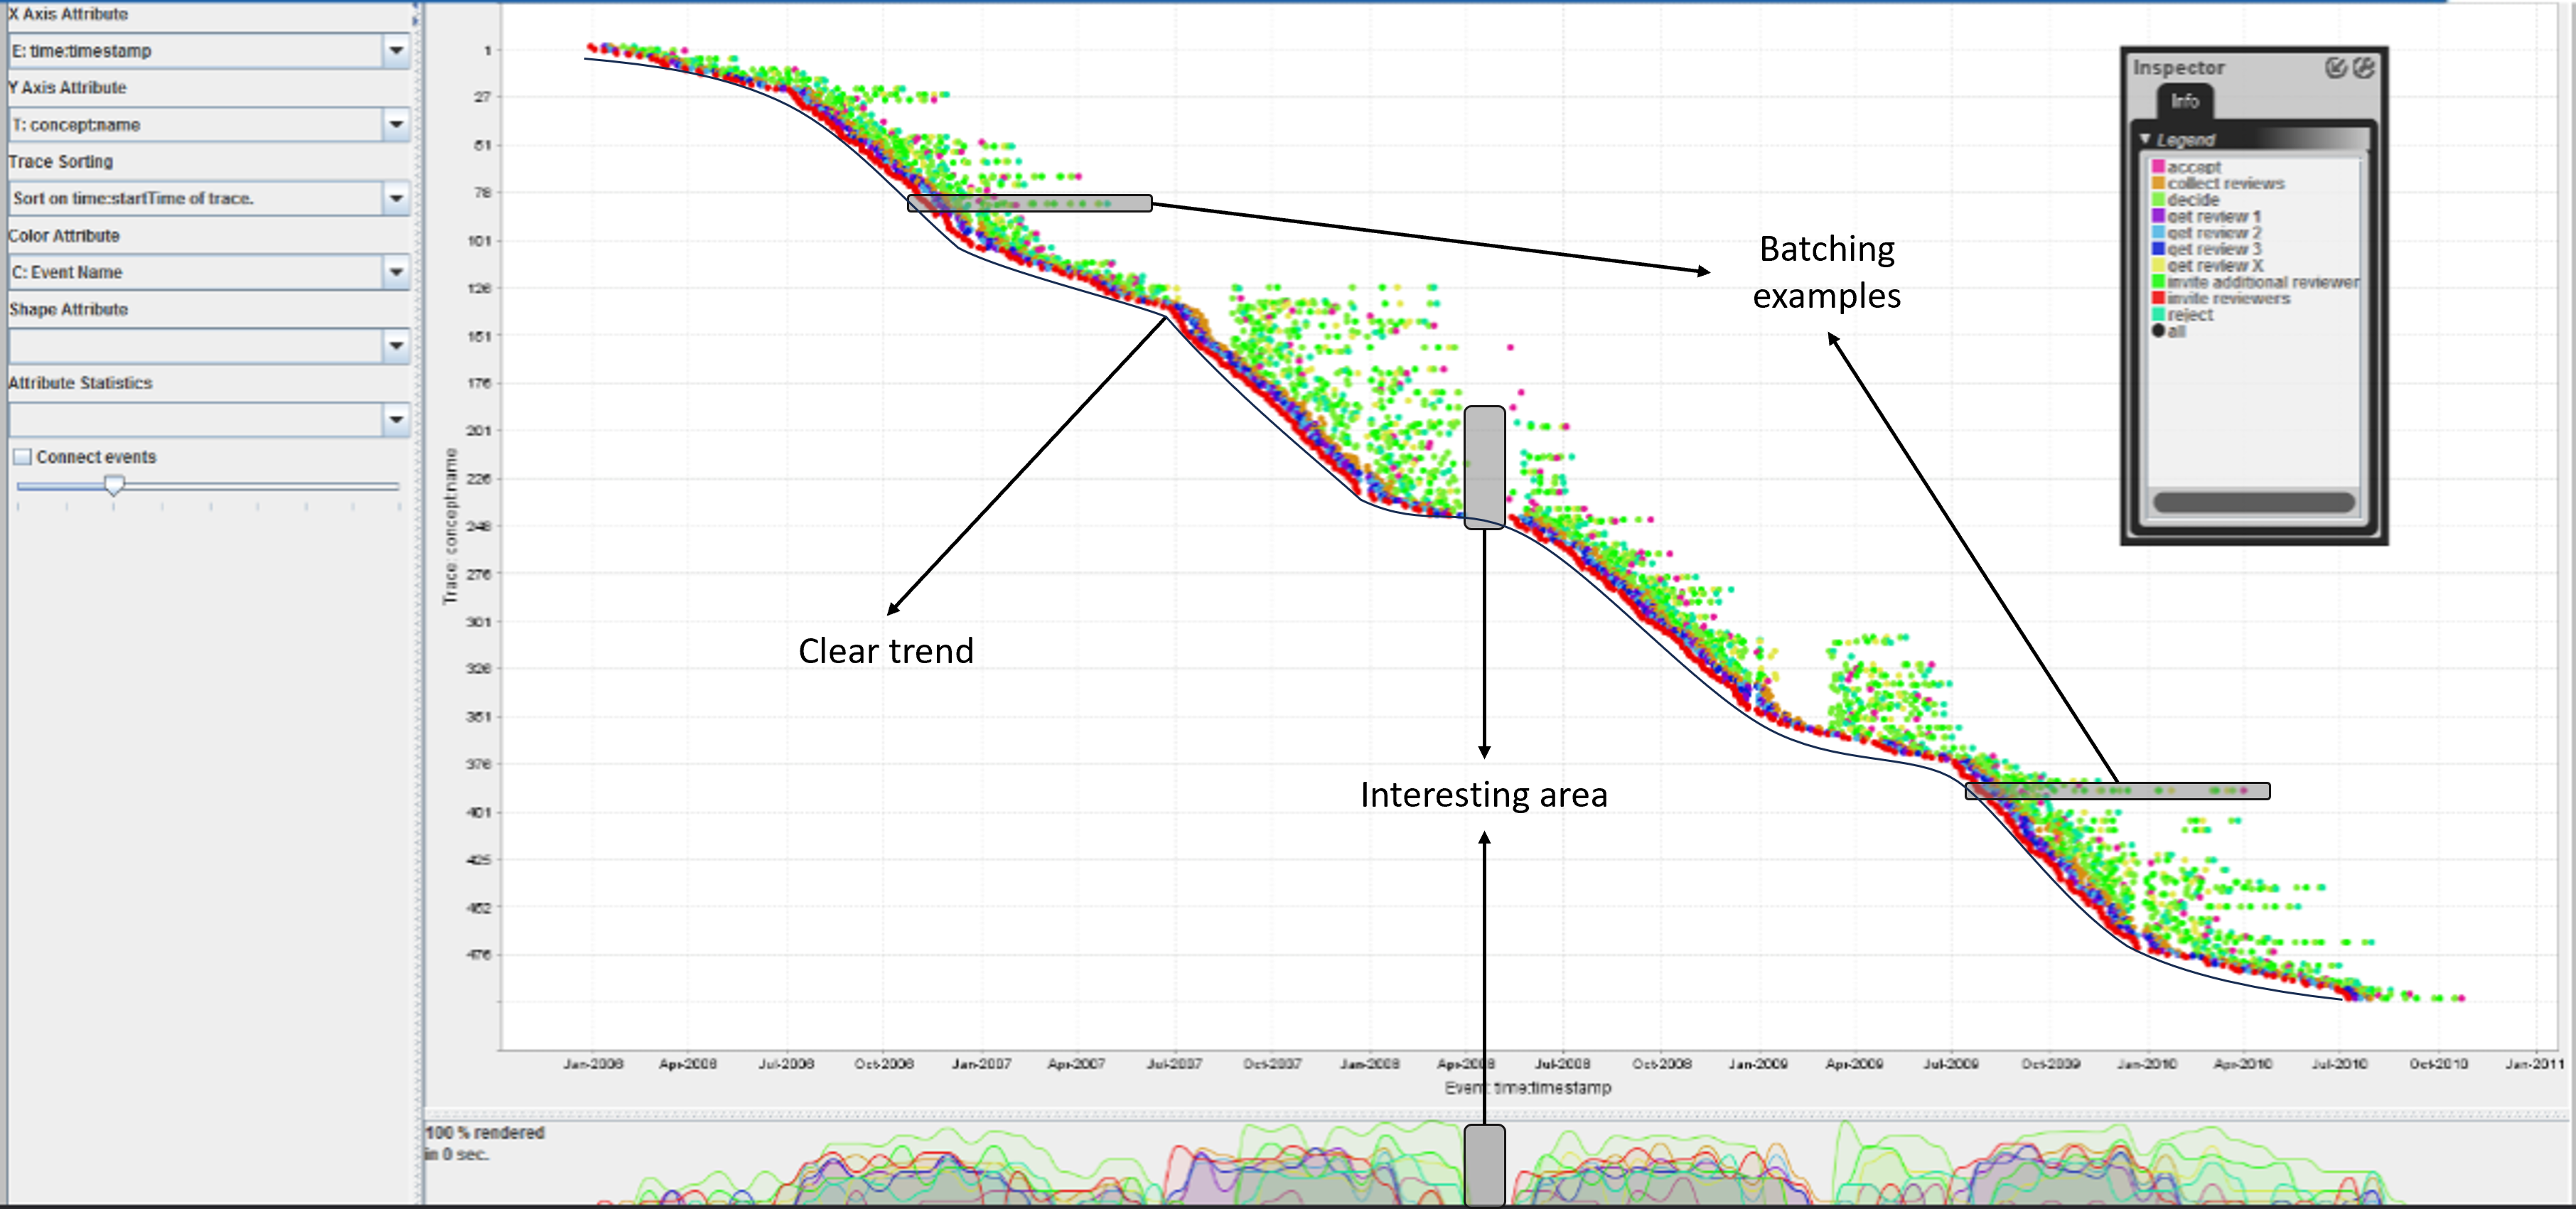
\includegraphics[width=\textwidth]{assets/visualization_and_extraction/event_data_visualization.png}
  \caption{Visualization of event data}
  \label{fig:2_event_data}
\end{figure}

\subsection{Characterizing individual features}

As a first step of actual data exploration, we are now going to look at which information we can get from a single data feature. In terms of tabular data: we're going to focus on a single column.

What kind of data we can derive from the feature, depends of course on the data type. Generally deriving features from other ones is of course done best when dealing with structured data. Here, we have two types from which we can derive different properties.

From \textbf{continuous features}, we can derive\sidenote{Investigation of individual \textbf{continuous} features}\renewcommand{\arraystretch}{1.5}

\begin{tabular}{@{}>{\raggedleft}m{0.2\textwidth} @{}>{\color{black}\centering:}m{0.025\textwidth} @{}>{\color{black}}m{0.775\textwidth}}
  count && Number of instances having this feature \\
  \% miss && Percentage of missing information {\color{gray}\footnotesize(how many instances don't have this feature)} \\
  card && Number of unique values (cardinality) \\
  min && Minimal value over all instances \\
  1\textsuperscript{st} qrt && 25\textsuperscript{th} percentile {\color{gray}\footnotesize(largest value of the quarter of instances having the lowest values)} \\
  mean && Average value over all instances \\
  median && Middle value of all instances \\
  3\textsuperscript{rd} qrt && 75\textsuperscript{th} percentile {\color{gray}\footnotesize(smallest value of the quarter of instances having the highest values)} \\
  max && Maximal value over all instances \\
  std. dev && Standard deviation over all instances
\end{tabular}


From \textbf{categorical features}, we can derive\sidenote{Investigation of individual \textbf{categorical} feature}\footnote{obvious: $\min$, $\max$, {\color{mathblue}mean}, etc. can't be computed}

\begin{tabular}{@{}>{\raggedleft}m{0.2\textwidth} @{}>{\color{black}\centering:}m{0.025\textwidth} @{}>{\color{black}}m{0.775\textwidth}}
  count && Number of instances having this feature \\
  \% miss && Percentage of missing information {\color{gray}\footnotesize(how many instances don't have this feature)} \\
  card && Number of unique values (cardinality) \\
  mode && Most common value \\
  mode frequ && Frequency of the mode \\
  mode \% && Percentage of the mode \\
  2\textsuperscript{nd}\,mode && Second most common value \\
  2\textsuperscript{nd}\,mode frequ && Frequency for the second mode \\
  2\textsuperscript{nd}\,mode \% && Percentage of the second mode
\end{tabular}

\begin{note}
To get a better idea of how to get these properties for all of the features, we will look at an example. Consider a table containing information about insurance claims fraud. The dataset contains 500 instances (claims) and a bunch of different features such as type, claim amount, etc. Now first, determine the data type of each feature, and then create one table for the numerical and one for the categorical features and fill it with the according information. The raw data can be found in \ref{fig:2_single_feature_example}.

\begin{figure}[h]
  \centering
  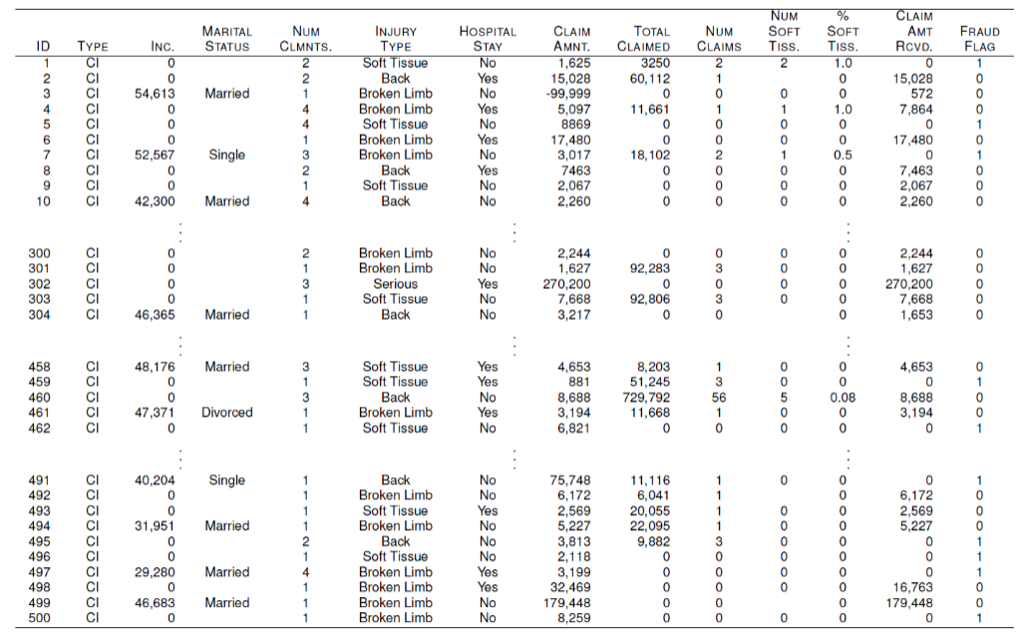
\includegraphics[width=\textwidth]{assets/visualization_and_extraction/single_feature_example/raw_data.png}
  \caption{Example for single feature investigation (insurance claim fraud)}
  \label{fig:2_single_feature_example}
\end{figure}

To investigate the raw data further, let's first extract the resulting feature-describing tables and then also visualize the data. More specifically for the visualization, we're going to show the distributions of the different features. Figure \ref{fig:2_distr_visualization} shows both the properties of the features and examplary plots.\end{note}
\begin{itemize}
  \item For finite amounts of possible feature classes, simply visualize the distribution as a bar diagram with the different classes as entries on the x-axis. The y-axis can either be the frequency or a percentage.
  \item For continuous features with continuous variables/infinitely many possible feature values, group items (\textbf{binning})\sidenote{Binning} and then visualize the resulting histogram.
\end{itemize}

\begin{figure}[H]
  \centering
  \subcaptionbox{Categorical features}{
    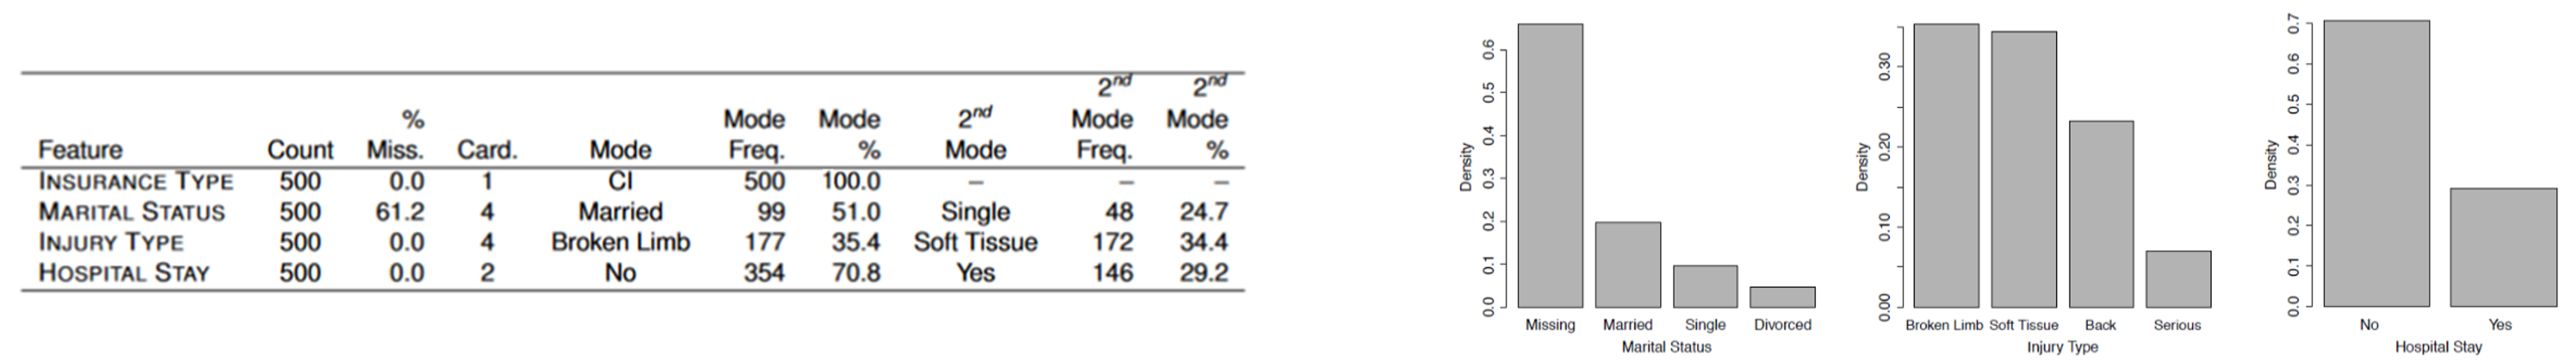
\includegraphics[width=\textwidth]{assets/visualization_and_extraction/single_feature_example/categorical.png}
  }
  \\\vspace*{0.25cm}
  \subcaptionbox{Numerical (continuous) features}{
    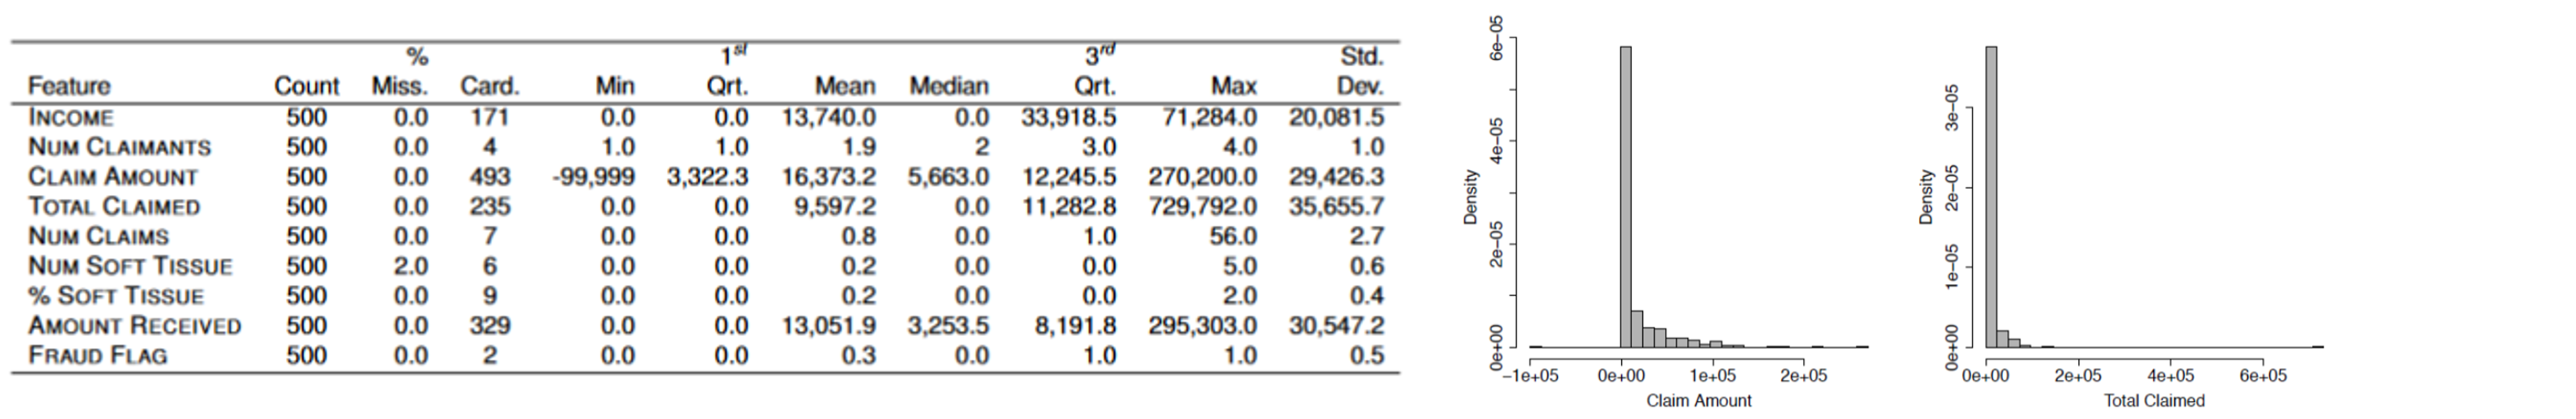
\includegraphics[width=\textwidth]{assets/visualization_and_extraction/single_feature_example/continuous.png}
  }
  \caption{Feature-discribing table and distribution visualization}
  \label{fig:2_distr_visualization}
\end{figure}

The binning comes with some challenges. When we select the amount of bins with evenly distributed width of each individual bin, we need to be aware not to \textbf{over- or underfit}\sidenote{Over- and underfitting for binning}. Examples can be found in \ref{fig:2_binning}. As one can see:
\begin{itemize}
  \item In the case of underfitting, the true function is not at all matched.
  \item In the case of overfitting, there exist very steep valeys, the provided data points are more learned by heart rather than abstracting to a function.
\end{itemize}

\begin{figure}[H]
  \centering
  \begin{subfigure}{0.32\textwidth}
    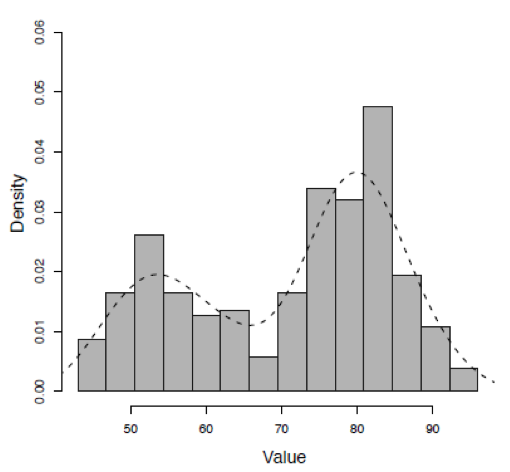
\includegraphics[width=\textwidth]{assets/visualization_and_extraction/single_feature_example/bin_good.png}
    \subcaption{Good approximation\\$\qquad \qquad14 \text{ \color{mathblue} bins}$}
  \end{subfigure}
  \begin{subfigure}{0.32\textwidth}
    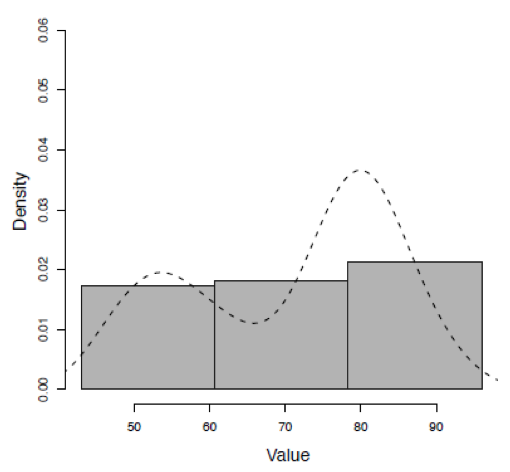
\includegraphics[width=\textwidth]{assets/visualization_and_extraction/single_feature_example/bin_underfitting.png}
    \subcaption{Underfitting\\$3 \text{ \color{mathblue} bins}$}
  \end{subfigure}
  \begin{subfigure}{0.32\textwidth}
    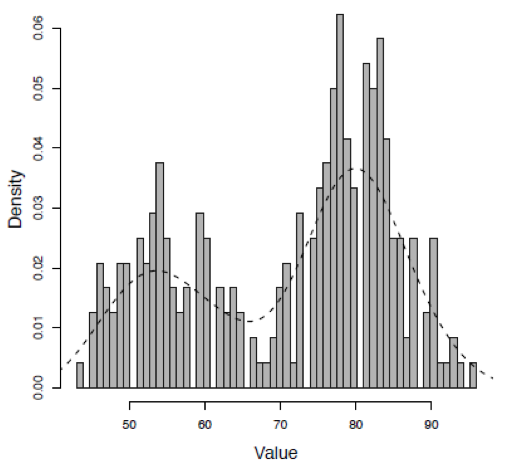
\includegraphics[width=\textwidth]{assets/visualization_and_extraction/single_feature_example/bin_overfitting.png}
    \subcaption{Overfitting\\$60 \text{ \color{mathblue} bins}$}
  \end{subfigure}
  \caption{Binning for continuous variables}
  \label{fig:2_binning}
\end{figure}

The histograms furthermore can show different types, as depicted in \ref{fig:2_histogram_types}.

\begin{figure}[H]
  \centering

  \begin{subfigure}{0.3\textwidth}
    \centering
    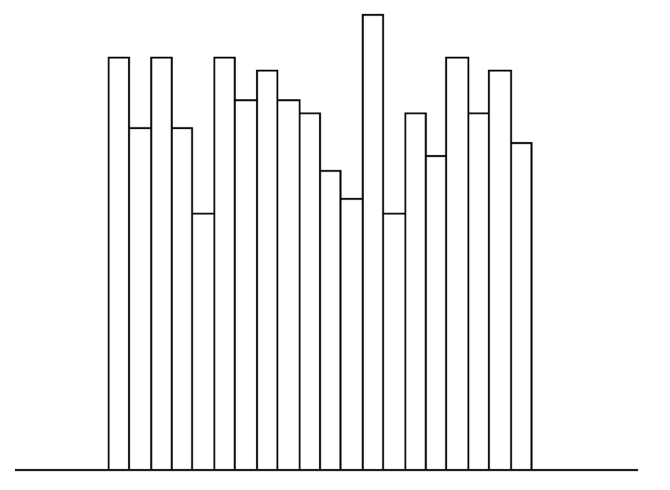
\includegraphics[width=0.7\textwidth]{assets/visualization_and_extraction/single_feature_example/distr_uniform.png}
    \subcaption{Uniform}
  \end{subfigure}\hspace*{0.01\textwidth}
  \begin{subfigure}{0.3\textwidth}
    \centering
    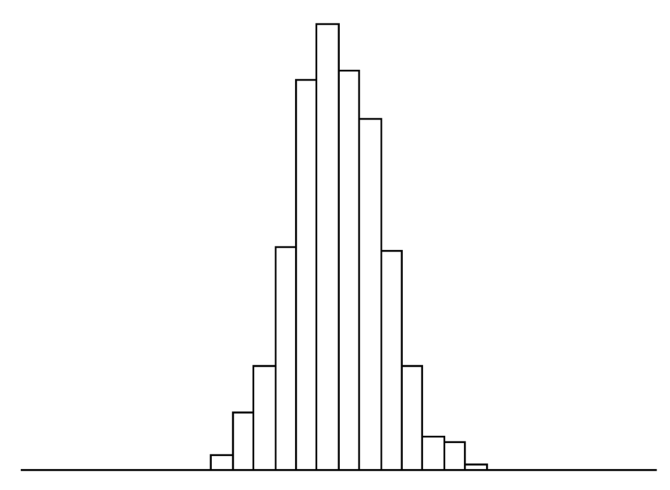
\includegraphics[width=0.7\textwidth]{assets/visualization_and_extraction/single_feature_example/distr_uni_normal.png}
    \subcaption{Unimodal, normal}
  \end{subfigure}\hspace*{0.01\textwidth}
  \begin{subfigure}{0.3\textwidth}
    \centering
    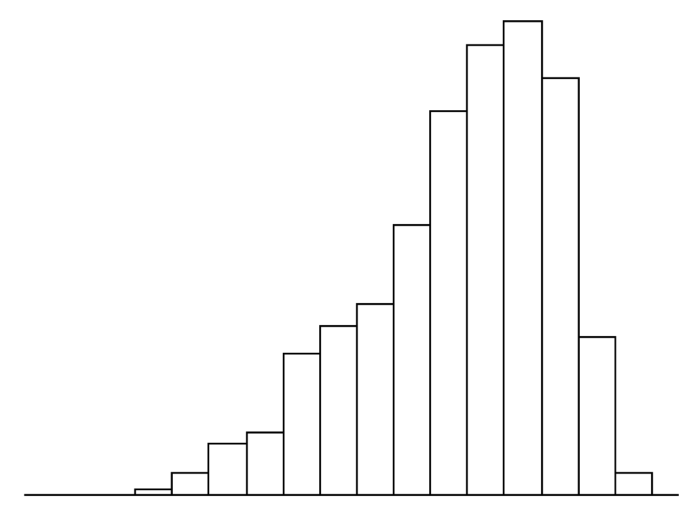
\includegraphics[width=0.7\textwidth]{assets/visualization_and_extraction/single_feature_example/distr_uni_right.png}
    \subcaption{Unimodal, skewed right}
  \end{subfigure}
  
  \vspace*{0.1cm}
  
  \begin{subfigure}{0.3\textwidth}
    \centering
    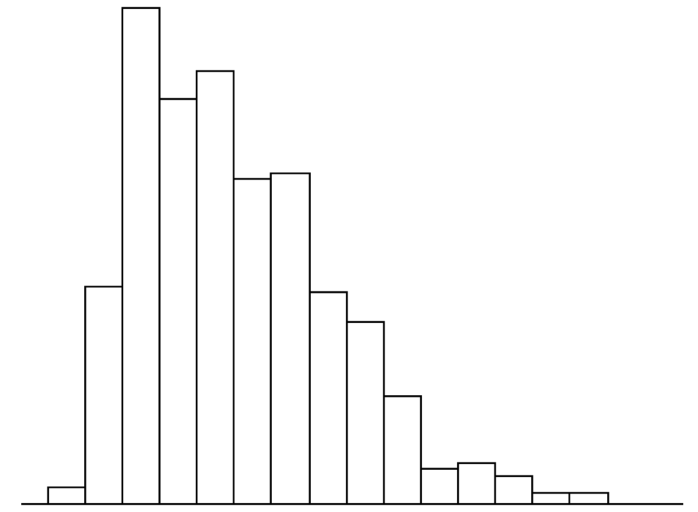
\includegraphics[width=0.7\textwidth]{assets/visualization_and_extraction/single_feature_example/distr_uni_left.png}
    \subcaption{Unimodal, skewed left}
  \end{subfigure}\hspace*{0.01\textwidth}
  \begin{subfigure}{0.3\textwidth}
    \centering
    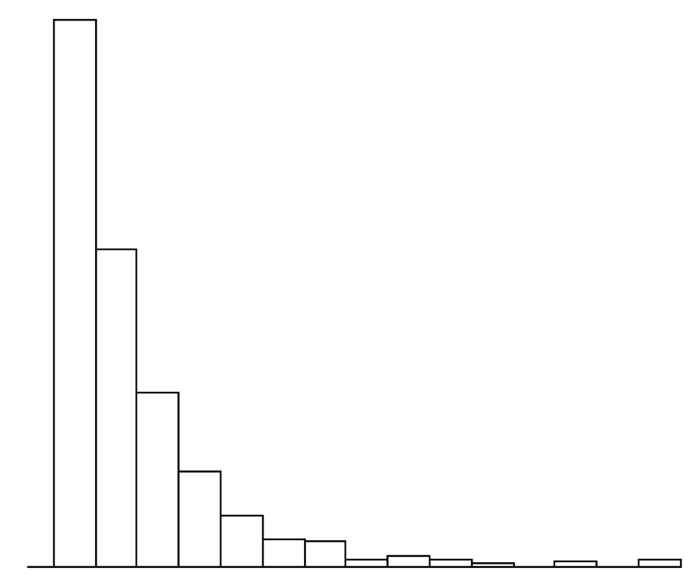
\includegraphics[width=0.7\textwidth]{assets/visualization_and_extraction/single_feature_example/distr_exp.png}
    \subcaption{Exponential}
  \end{subfigure}\hspace*{0.01\textwidth}
  \begin{subfigure}{0.3\textwidth}
    \centering
    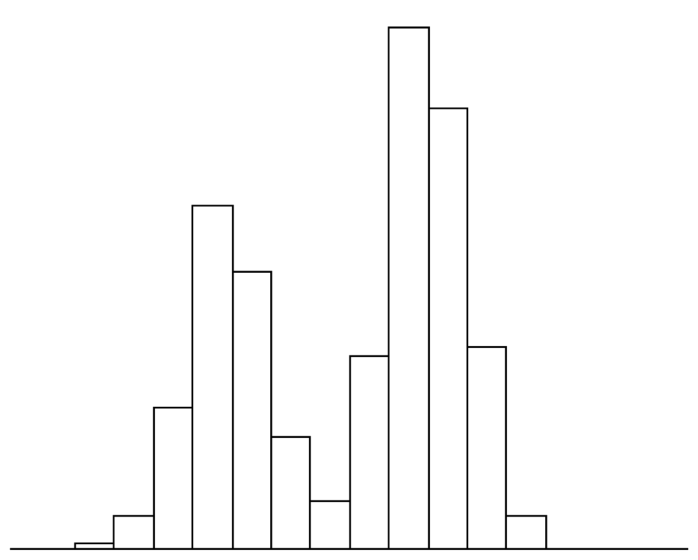
\includegraphics[width=0.7\textwidth]{assets/visualization_and_extraction/single_feature_example/distr_multi.png}
    \subcaption{Multimodal}
  \end{subfigure}

  \caption{Histogram types}
  \label{fig:2_histogram_types}
\end{figure}

Here are some further notes on the types:
\begin{itemize}
  \item \textbf{Uniform}\sidenote{Uniform} means all items have the same likelyhood (within a range).
  \item \textbf{Unimodal}\sidenote{Unimodal} means we have one peak (can be tilted to one side), whereas \textbf{multimodal}\sidenote{Multimodal} means there are multiple distinct ones.
  \item \textbf{Exponential}\sidenote{Exponential} means we have an exponential descrease in the likelihood over all instances.
\end{itemize}


\subsubsection*{Normal distribution}

One of the types mentioned, we're now gonna investigate a bit further. The \textbf{normal distribution}\sidenote{Normal distribution} is described by two important variables, whose effects on the distribution are shown in \ref{fig:2_normal}:
\begin{itemize}
  \item The \textbf{mean}\sidenote{Mean}$\mu$, so the expected value also characterizing the peak, and
  \item The \textbf{standard deviation}\sidenote{Standard deviation}$\sigma$ characterizing how narrow the peak, or the distribution around the peak, is.
\end{itemize}

\begin{figure}[H]
  \centering
  \subcaptionbox{Variation of mean $\mu$}{
    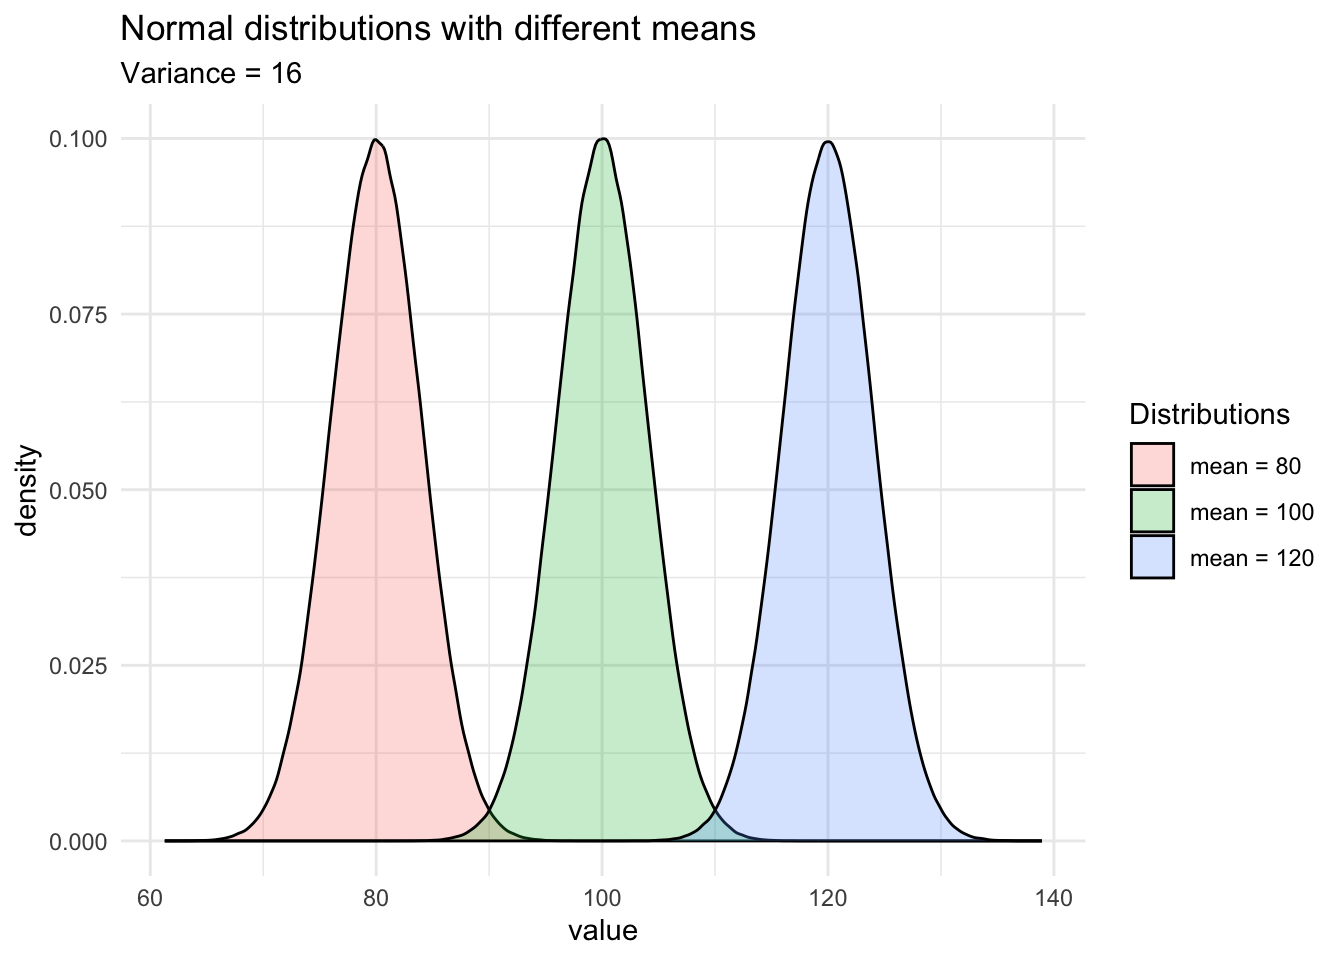
\includegraphics[width=0.4\textwidth]{assets/visualization_and_extraction/norm_mean.png}
  }
  \hspace*{0.05\textwidth}
  \subcaptionbox{Variation of standard deviation $\sigma$}{
    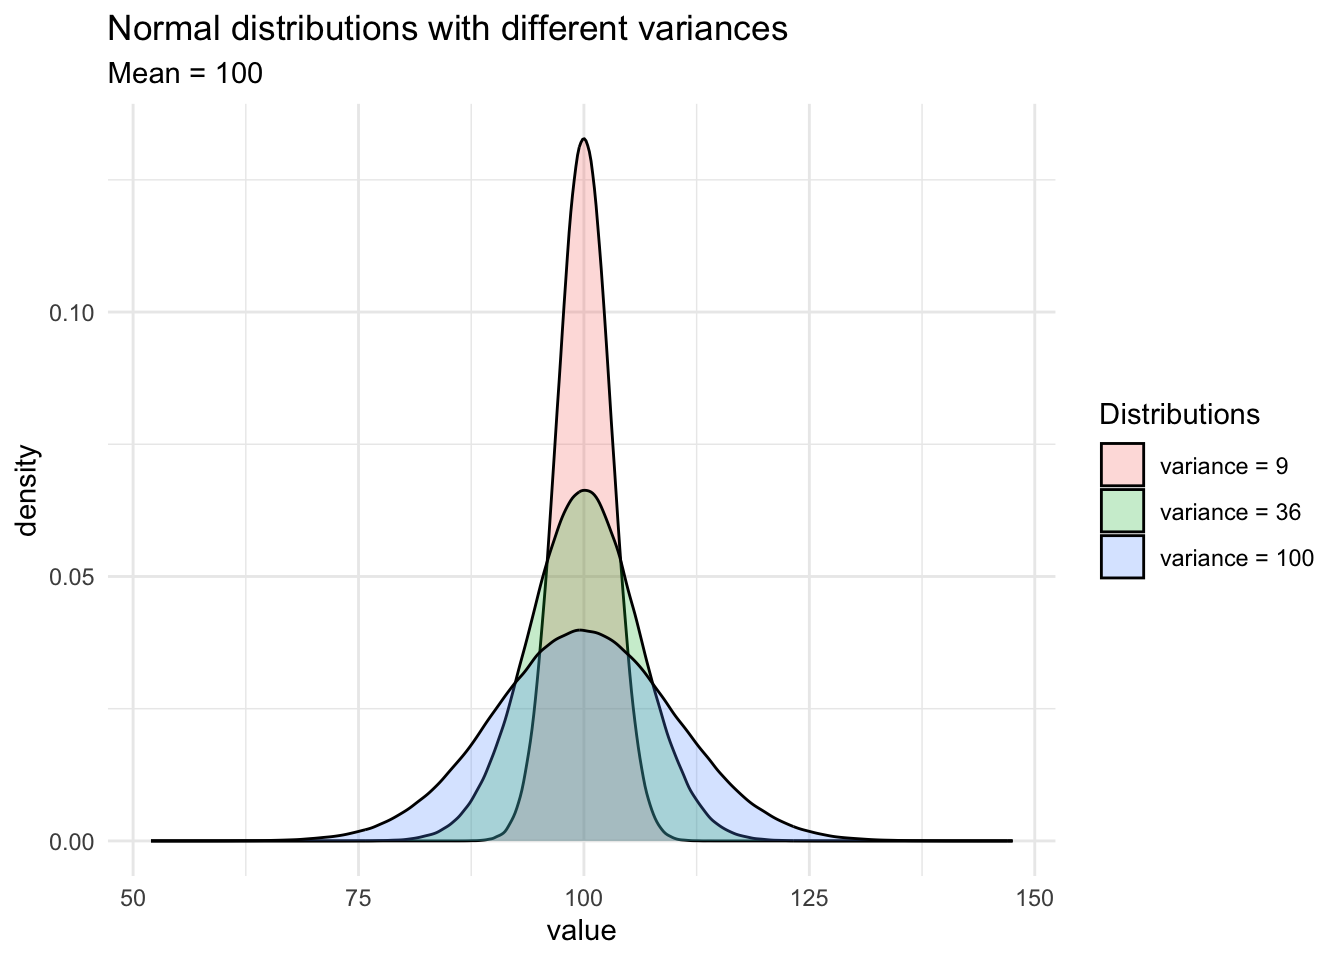
\includegraphics[width=0.4\textwidth]{assets/visualization_and_extraction/norm_var.png}
  }
  \caption{Normal distribution}
  \label{fig:2_normal}
\end{figure}

The normal probability distribution over $x$ is defined as:
\begin{align*}
  x \sim&\, \mathcal{N}(\mu, \sigma) \\
  p(x) = &\,\frac{1}{\sqrt{2\pi \sigma^2}} \cdot \exp\left[ -\frac{1}{2}\left(\frac{x-\mu}{\sigma}\right)^2 \right]
\end{align*}

Interesting are now precise areas we instantly know something about. The $68$-$95$-$99.7$-rule\sidenote{$68$-$95$-$99.7$-rule} tells us, as depicted in \ref{fig:2_three_sigma}.
\begin{itemize}
  \item $68\%$ of all observations will be within $1\sigma$-distance of the mean,
  \item $95\%$ of all observations will be within $2\sigma$-distance of the mean, and
  \item $99.7\%$ of all observations will be within $3\sigma$-distance of the mean
\end{itemize}

\begin{figure}[H]
  \centering
  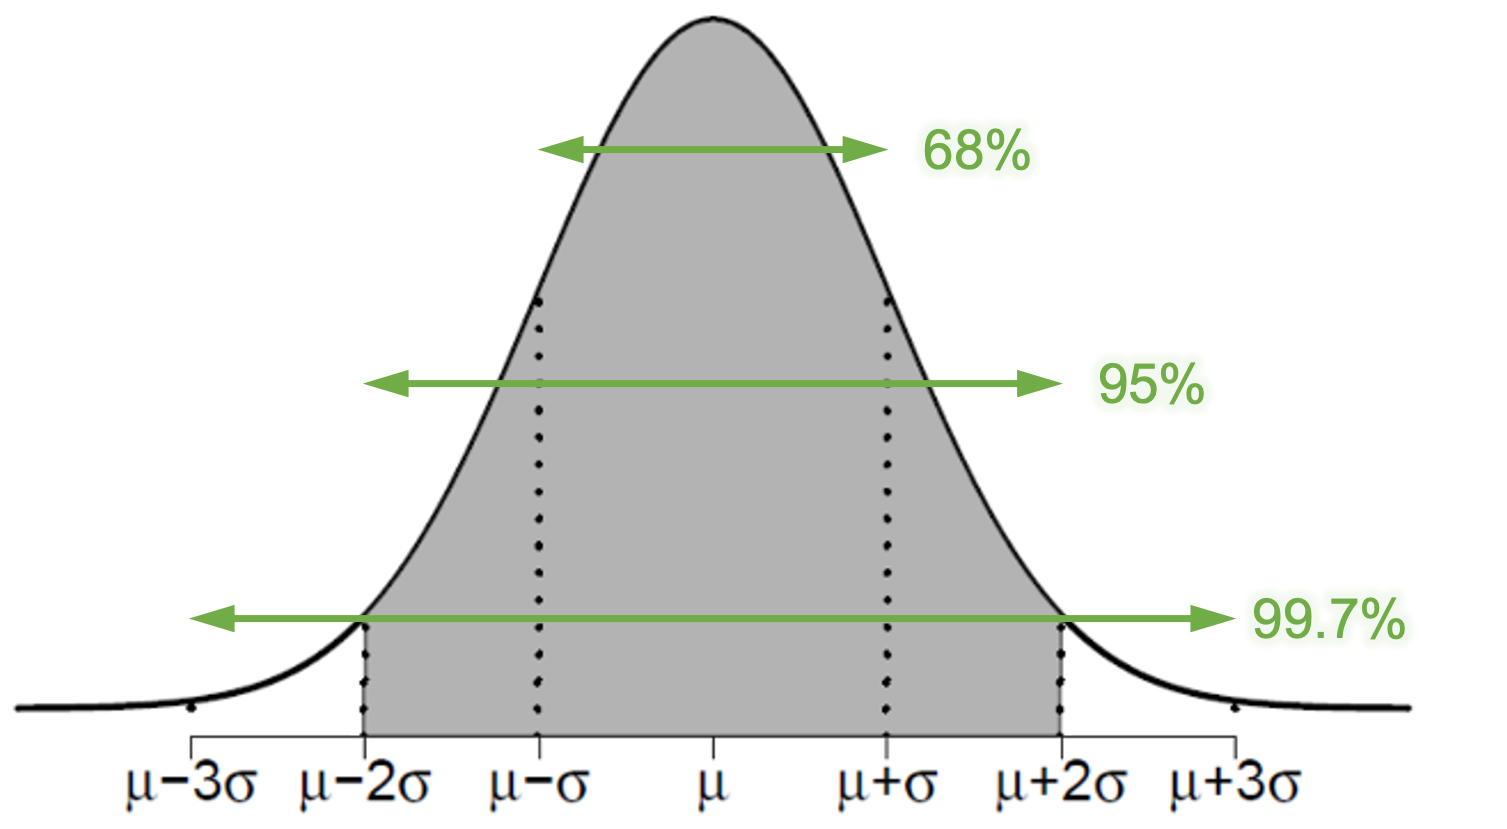
\includegraphics[width=0.5\textwidth]{assets/visualization_and_extraction/norm_rule.png}
  \caption{$68$-$95$-$99.7$-rule}
  \label{fig:2_three_sigma}
\end{figure}

From this rule, we can now derive probabilities for different events. \begin{note}Consider the following examples, also visualized in \ref{fig:2_three_sigma_examples}:
\begin{itemize}
  \item Example 1 is interested in the amount of defects for some produced item. The \textbf{tolerance} can be defined as within the $2\sigma$-range, so with:
  \begin{itemize}
    \item \textbf{LSL} (lower spcification limit)\sidenote{LSL} at $\mu-2\sigma$, meaning only $2.5\%$ of the instances have a larger deviation into the negative direction from the mean than this limit, and
    \item \textbf{USL} (upper spcification limit)\sidenote{USL} at $\mu-2\sigma$, meaning only $2.5\%$ of the instances have a larger deviation into the positive direction from the mean than this limit.
  \end{itemize}
  Combined, $100\%-2.5\%-2.5\%=95\%$ have a deviation from the mean lying withing the defined range.
  \item Example 2 is interested in how many deliveries are too late. Therefore, it \textbf{only} defined an \textbf{upper bound} with the USL at $\mu+2\sigma$. This means, $100\%-2.5\%=97.5\%$ of the deliveries are not to late.
\end{itemize}
\end{note}

\begin{figure}[H]
  \centering
  \subcaptionbox{Example 1 (defect tolerance)}{
    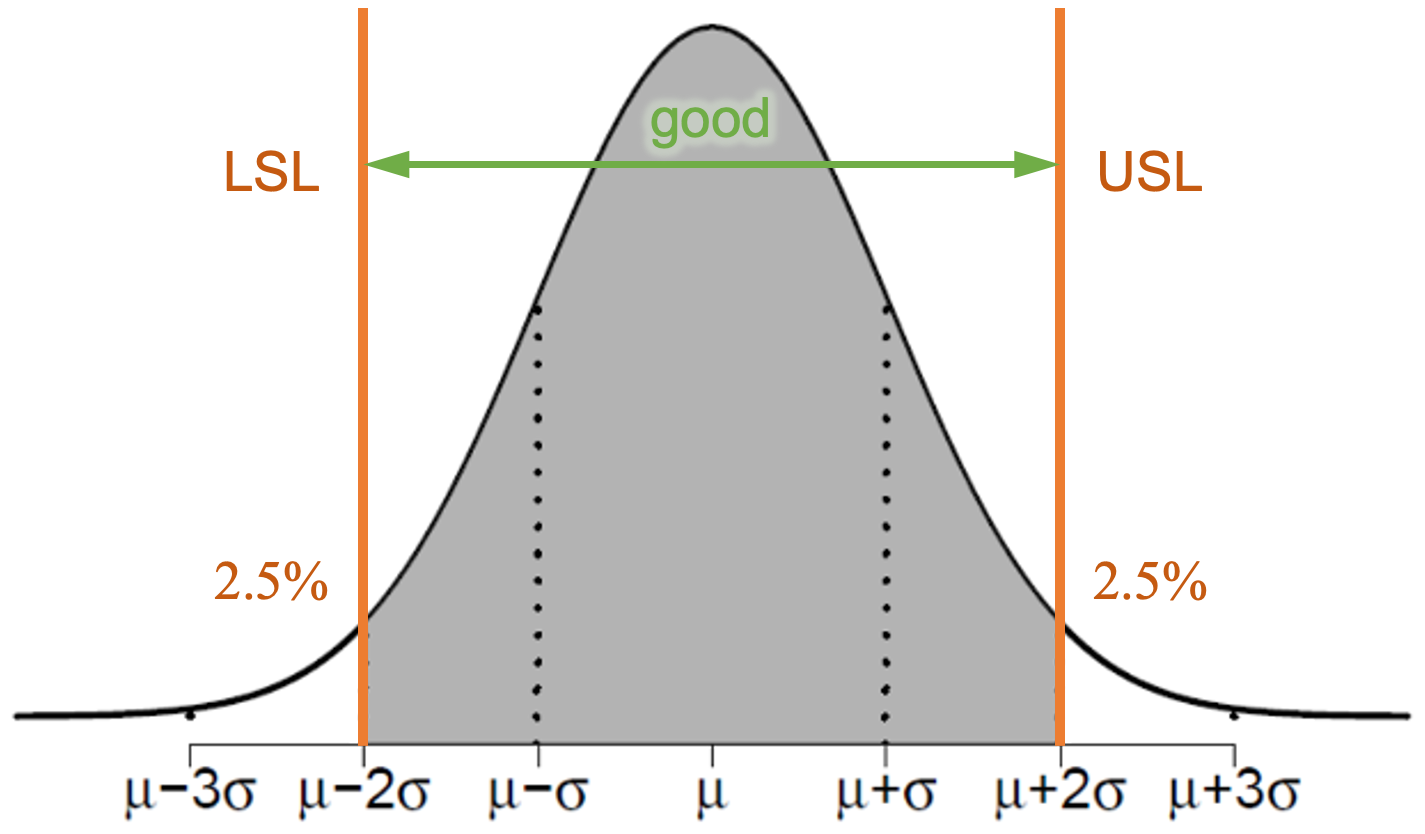
\includegraphics[width=0.4\textwidth]{assets/visualization_and_extraction/norm_rule_example_1.png}
  }
  \hspace*{0.05\textwidth}
  \subcaptionbox{Example 2 (delivery times)}{
    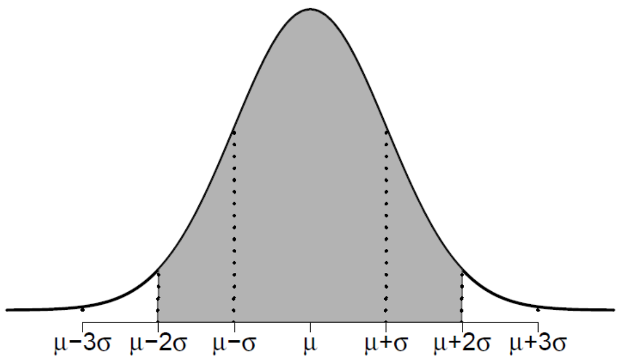
\includegraphics[width=0.4\textwidth]{assets/visualization_and_extraction/norm_rule_example_2.png}
  }
  \caption{Examples for $68$-$95$-$99.7$-rule}
  \label{fig:2_three_sigma_examples}
\end{figure}

Furthermore, the rule also introduces the term of \textbf{six sigma} or also lean six sigma. It basically means that processes operating with "Six Sigma quality" are assumed to have $< 3.4$ defects per million instances, so $\Pr(\text{error})=0.0000034$. It characterizes a process improvement approach. This likelihood is a combination of $\pm6\sigma$ tolerance and a "drift" of $\pm1.5\sigma$. 

\begin{figure}[H]
  \centering
  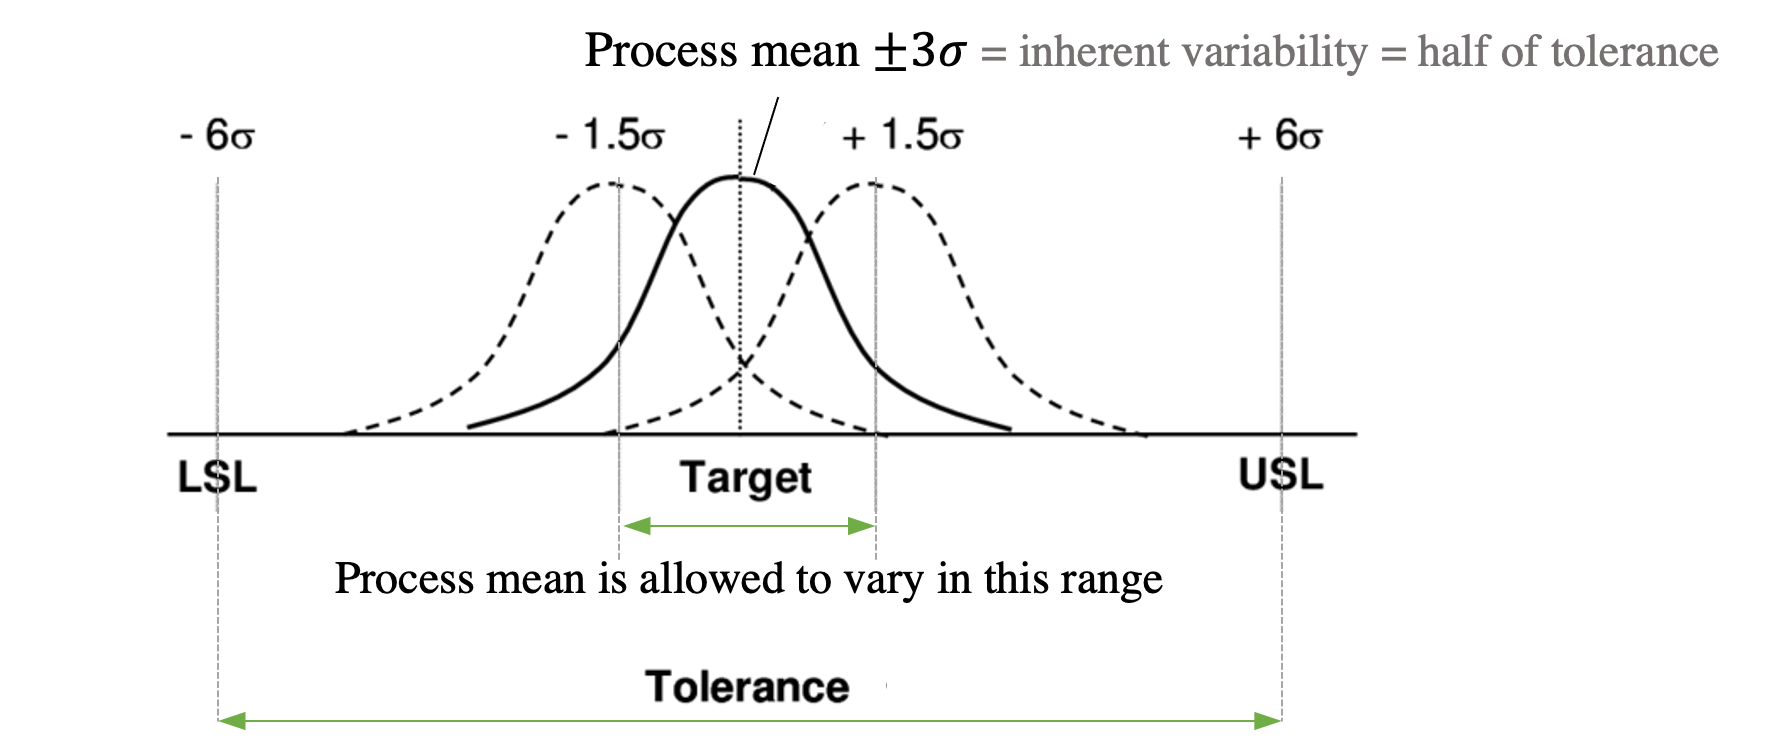
\includegraphics[width=0.6\textwidth]{assets/visualization_and_extraction/lean_six_sigma.png}
  \caption{Lean six sigma}
  \label{fig:2_lean_six_sigma}
\end{figure}


\subsection{Data quality}

In the introduction, we already looked at some key challenges regarding data quality. In this subsection, we will investigate and search solutions for the some of the following typical data quality problems in detail:
\begin{itemize}
  \item \textbf{Incompleteness} - missing instances or attributes
  \item \textbf{Invalidity} - impossible values
  \item \textbf{Inconsitency} - conflicting values
  \item \textbf{Imprecision} - approximates or rounded values
  \item \textbf{Outdated} - values based on old observations
\end{itemize}

For that, we will take a look at missing, invalid, unlikely, and outlier values.

\subsubsection*{Missing values}
Imagine different missing features\sidenote{Missing features} of some instances. Since some data is missing, we need to deal with this in some way. Here are the possible options:
\begin{enumerate}
  \item Remove feature completely (for all instances)
  \item Only consider instsances that have a value (this is done for per-feature-evaluation)
  \item Remove all instances that have one of the features missing
  \item Repair missing features (imputation)
\end{enumerate}

The problem setting and the possible solutions are visualized in \ref{fig:2_missing_values}.

\begin{figure}[h]
  \centering
  \begin{subfigure}{0.4\textwidth}
    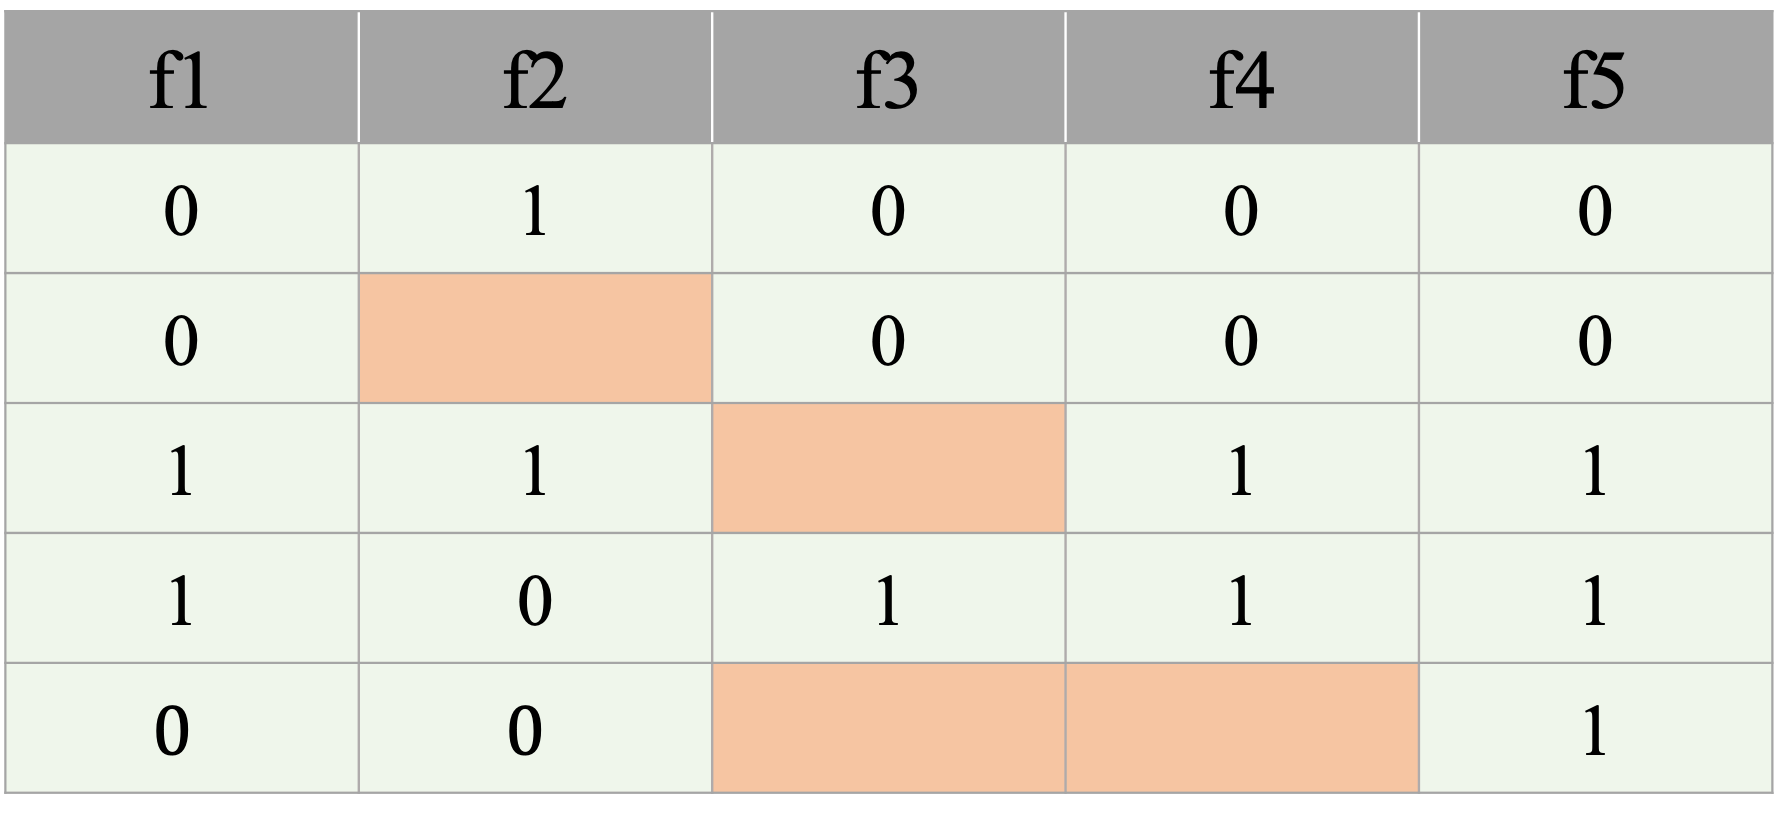
\includegraphics[width=\linewidth]{assets/visualization_and_extraction/problem_missing_values.png}
    \caption{Problem setting}
  \end{subfigure}\\
  \vspace*{0.5cm}
  \begin{subfigure}{0.7\textwidth}
    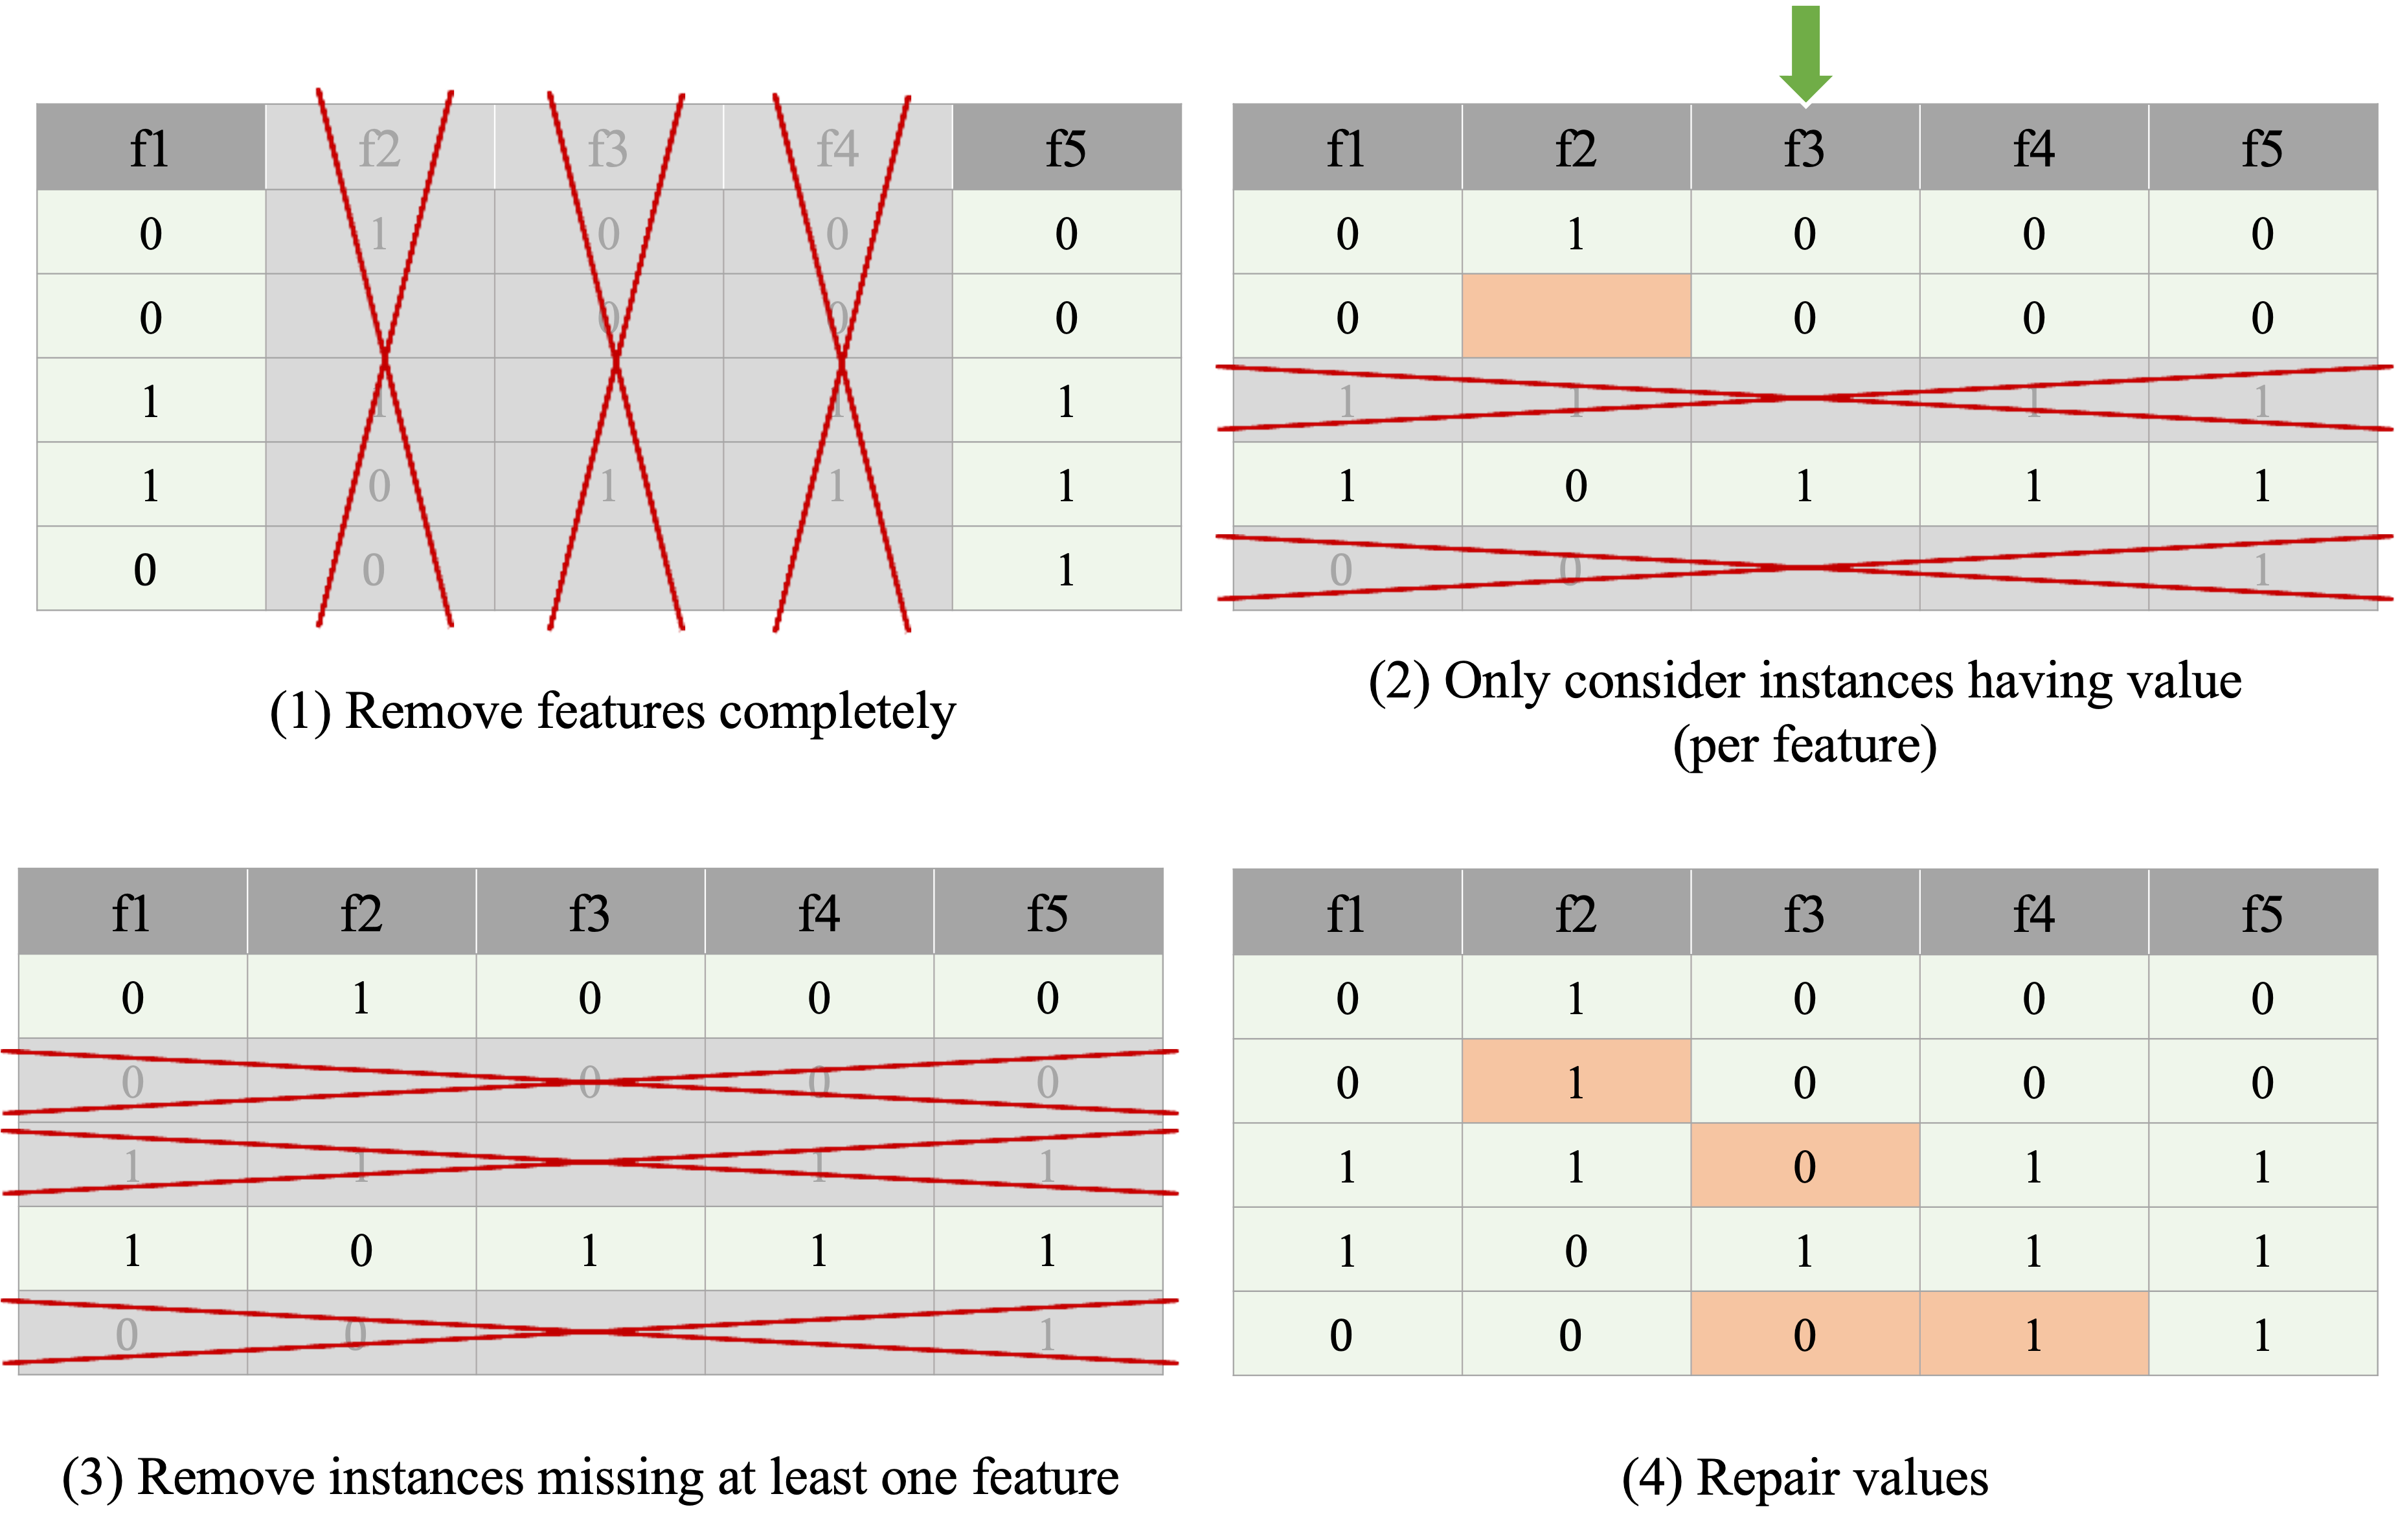
\includegraphics[width=\linewidth]{assets/visualization_and_extraction/solution_missing_values.png}
    \caption{Possible solutions}
  \end{subfigure}
  \caption{Missing values}
  \label{fig:2_missing_values}
\end{figure}

\subsubsection*{Impossible values}
The next typical challenge are impossible values\sidenote{Impossible values} that by some mistake were entered as data. Examples are:
\begin{itemize}
  \item Wrong date format: instead of \textcolor{mathblue}{2018-10-18}, we would have \textcolor{mathblue}{18-10-2018}
  \item Completely impossible date or time: \textcolor{mathblue}{2018-13-51}, \textcolor{mathblue}{23:61}
  \item There can be spelling errors, for example for colors: \textcolor{mathblue}{Bllue}
  \item The data type might not make sense with the feature, like number of members as a float: \textcolor{mathblue}{6.5 member}
\end{itemize}

The handling of this problem is solved just as for missing features.

\subsubsection*{Unlikely values}
In contrast to impossible values, unlikely values are theoretically possible, but just not common to appear. Examples are:
\begin{itemize}
  \item Age: $123$ is rather unlikely, but possible
  \item Price: $120.000\$$ in a store where the other prices lie in the range of $5\$$ to $150\$$
  \item Dates: even on dates, where one would usually expect a uniform distribtion over months and days, days $1$ to $12$ are more frequent than days $13$ to $31$\footnote{NOT the case anymore if date format \textcolor{mathblue}{DD-MM-YYYY} and \textcolor{mathblue}{MM-DD-YYYY} are mixed}
\end{itemize}
Whether a value is unlikely or not is identified based on \textbf{domain knowledge}\sidenote{Unlikely values, domain knowledge}. They can then be further investigated to see, whether the unlikely value is acutally valid.


\subsubsection*{Outlier values}
In contrast to unlikely values, \textbf{outlier values}\sidenote{Outlier values} are identified based on the distribution. 

An especially popular technique to visualize distributions and outliers are \textbf{box plots}\sidenote{Box plot}. They were first introduced by John Tukey in the book "Exploratory data analysis" in 1977. Figure \ref{fig:2_box_plot} shows the properties visualized by a box plot and also how to construct one given a data set. 

\begin{figure}[h]
  \centering
  \subcaptionbox{Properties on a box plot}{
    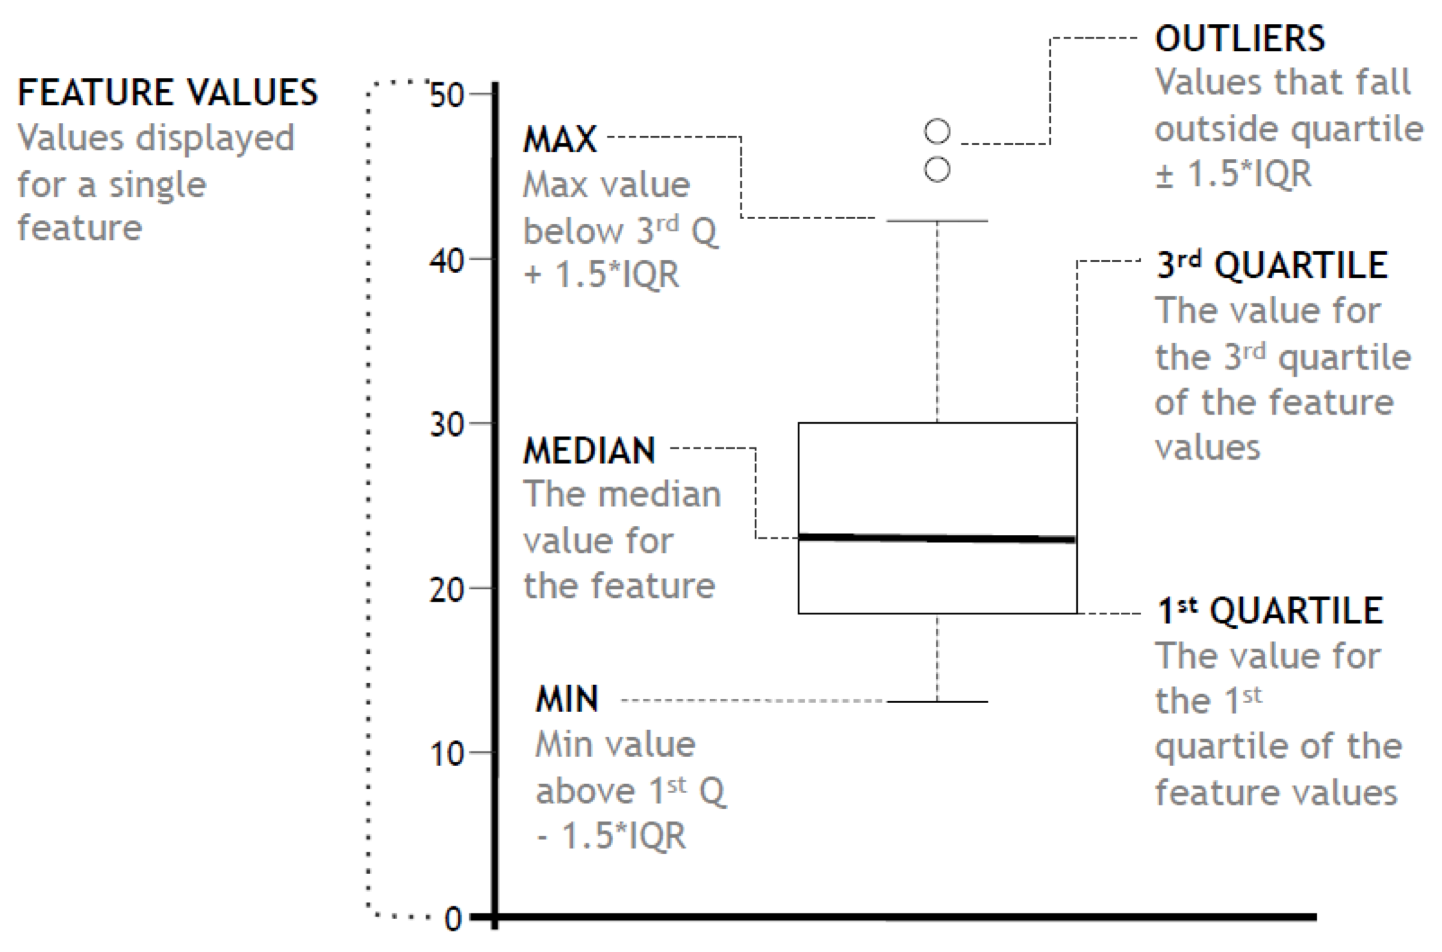
\includegraphics[height=4.9cm]{assets/visualization_and_extraction/box_properties.png}
  }
  \hspace*{0.05\textwidth}
  \subcaptionbox{Construction of a box plot}{
    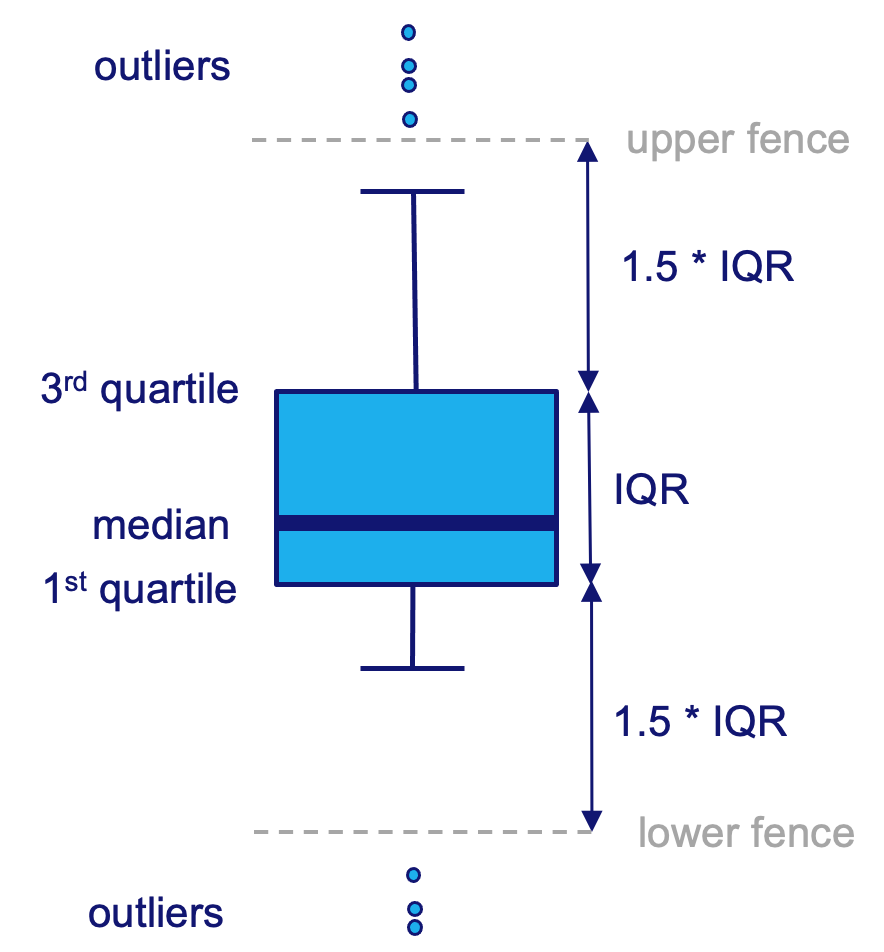
\includegraphics[height=4.9cm]{assets/visualization_and_extraction/box_construction.png}
  }
  \caption{Box plot}
  \label{fig:2_box_plot}
\end{figure}

Let's first take a look at the properties one can see in the box diagram. 
\begin{itemize}
  \item The \textbf{median} value is depicted by the "Bar" in the center.
  \begin{itemize}
    \item The median is the "middle" value, so the number halway between lowest and highest number.
  \end{itemize}
  \item The \textbf{IQR}\sidenote{IQR}, so the interquartile range, covering $50\%$ of the "middle instances" is depicted by the "Box".
  \begin{itemize}
    \item The first quartile is the number halway between lowest and middle number, the third halway between middle and highest number.
    \item The IQR is the distance between first and third quartile.
  \end{itemize}
  \item The upper whisker indicates the \textbf{maximal} value below the $3^{\text{\color{mathblue}rd}} \text{\color{mathblue} quartile} + 1.5\cdot IQR$, whereas
  \item The lower whisker indicates the \textbf{minimal} value above the $1^{\text{\color{mathblue}st}} \text{\color{mathblue} quartile} - 1.5\cdot IQR$.
  \item Finally, the \textbf{outliers} are drawn separately.
\end{itemize}

The description already contained a bit of the construction details, which will now be explained in more detail with an example. Consider the (already ordered) data set:
\begin{align*}
  \{
  \text{\textcolor{mathblue}{\small 
  {\tiny \color{gray} 1: }1, {\tiny \color{gray} 2: }2, {\tiny \color{gray} 3: }5, {\tiny \color{gray} 4: }7, {\tiny \color{gray} 5: }8, {\tiny \color{gray} 6: }8, {\tiny \color{gray} 7: }9, {\tiny \color{gray} 8: }9, {\tiny \color{gray} 9: }9, {\tiny \color{gray} 10: }10, {\tiny \color{gray} 11: }10, {\tiny \color{gray} 12: }10, {\tiny \color{gray} 13: }11, {\tiny \color{gray} 14: }12, {\tiny \color{gray} 15: }14, {\tiny \color{gray} 16: }19, {\tiny \color{gray} 17: }23 
  }}
  \}
\end{align*}
 
Then we construct the box diagram like this:
\begin{itemize}
  \item The median value is $9$ \textcolor{gray}{\tiny(at position 9)}.
  \item The first quatile has the value $8$ \textcolor{gray}{\tiny(at position 5)}, the third one has the value $11$ \textcolor{gray}{\tiny(at position 13)} resulting in an $IQR = 11-8 = 3$.
  \item This means we have an upper fence $11 + 1.5\cdot3 = 15.5$, and the upper whisker as the maximum value below this fence at $14$ \textcolor{gray}{\tiny(position 15)}.
  \item The lower fence has the value $8 - 1.5\cdot3 = 3.5$, the lower whisker therefore the minimum value above this fence value at $5$ \textcolor{gray}{\tiny(position 3)}.
  \item Finally, the outliers are $1, 2, 19, 23$ \textcolor{gray}{\tiny(position 1, 2, 16, 17)}.
\end{itemize}
Those are all the necessary components to construct the box diagram.

Now, one final detail about box diagrams and also the topic of this paragraph is the handling of the outliers. They can first be removed (meaning remove values above and below the upper and lower fences), and their existance can be indicated by claming the removed values to these thresholds. The process is shown in \ref{fig:2_box_plot_outlier_handling}.

\begin{figure}[h]
  \centering
  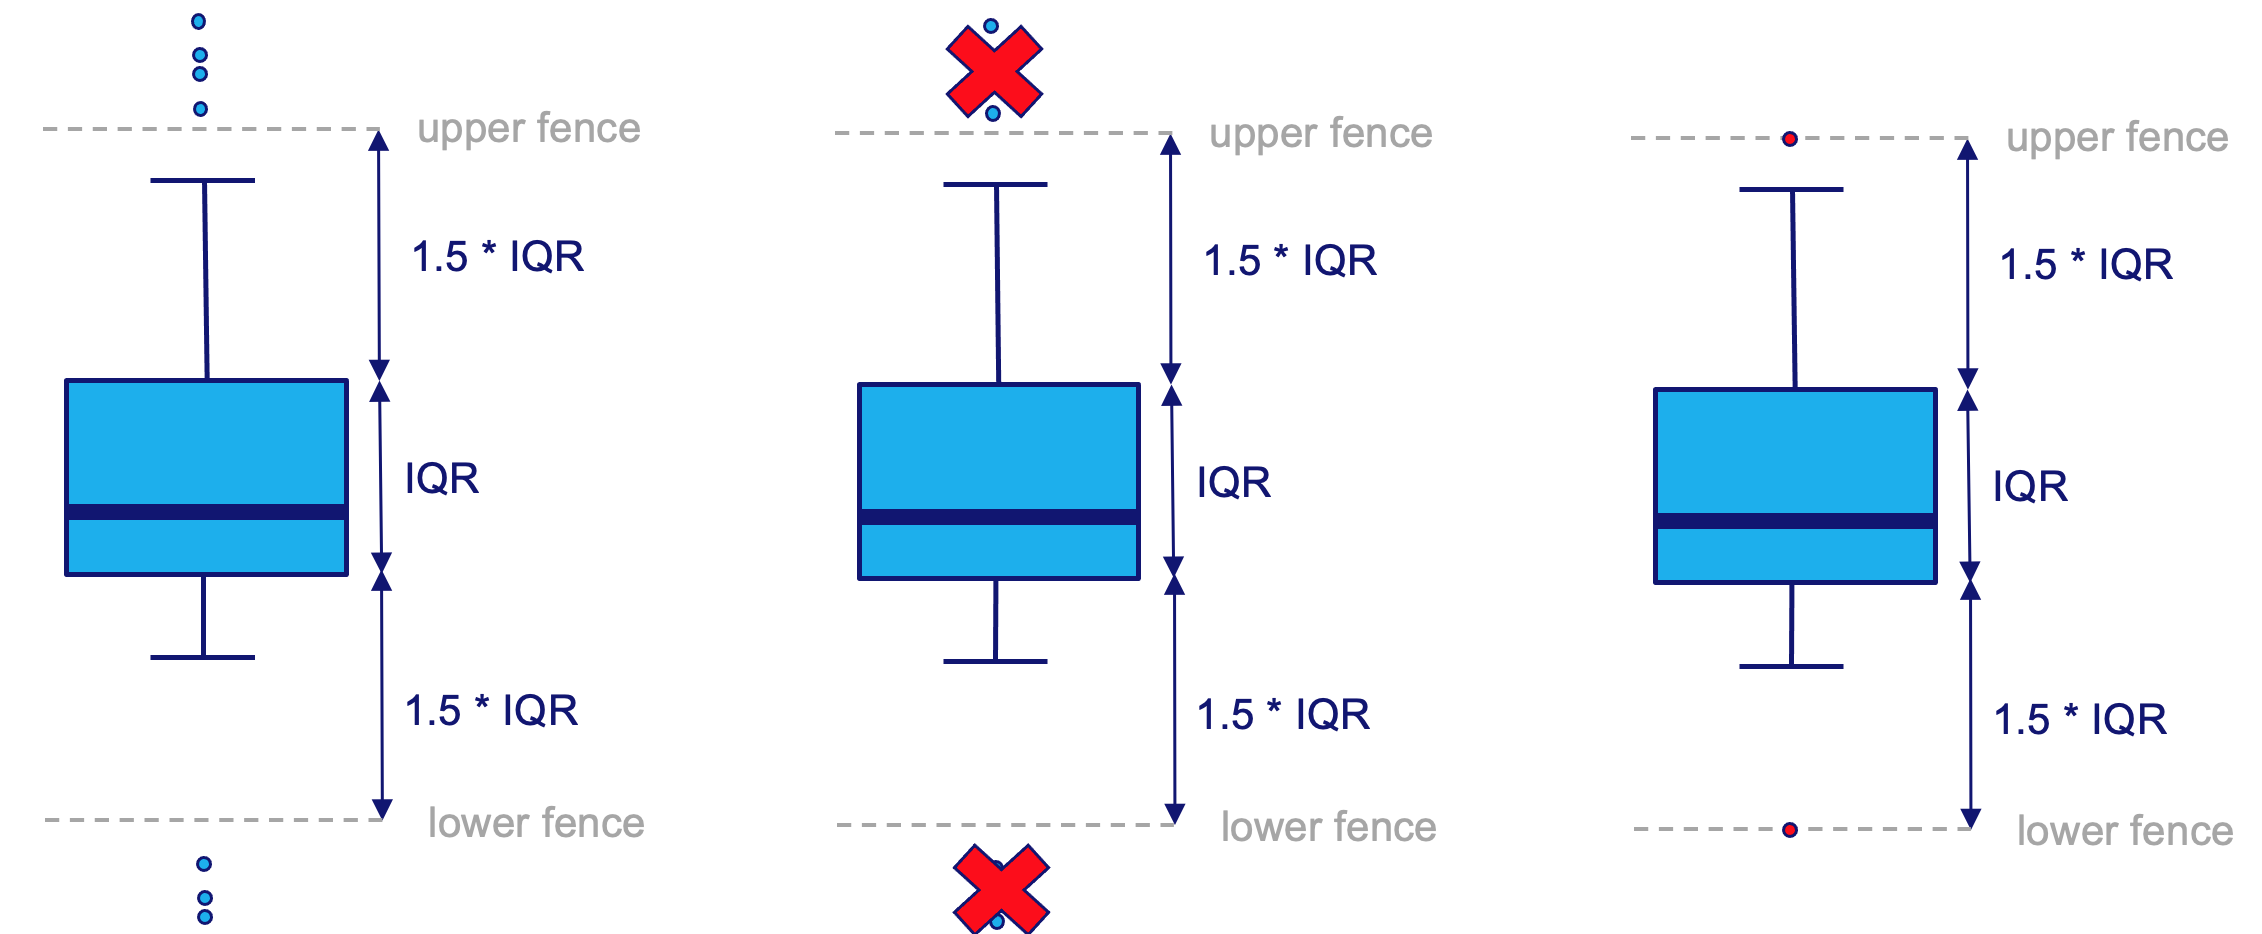
\includegraphics[height=4.5cm]{assets/visualization_and_extraction/box_outliers.png}
  \caption{Handling outliers in box plots}
  \label{fig:2_box_plot_outlier_handling}
\end{figure}

\subsection{Showing relations among features}
\subsection{Preparing for analysis}
\subsection{Good and poor visualizations}
